\section{Anhang}
	
	\subsection{Graphen}
	\begin{figure}[!ht]
		\centering								 
		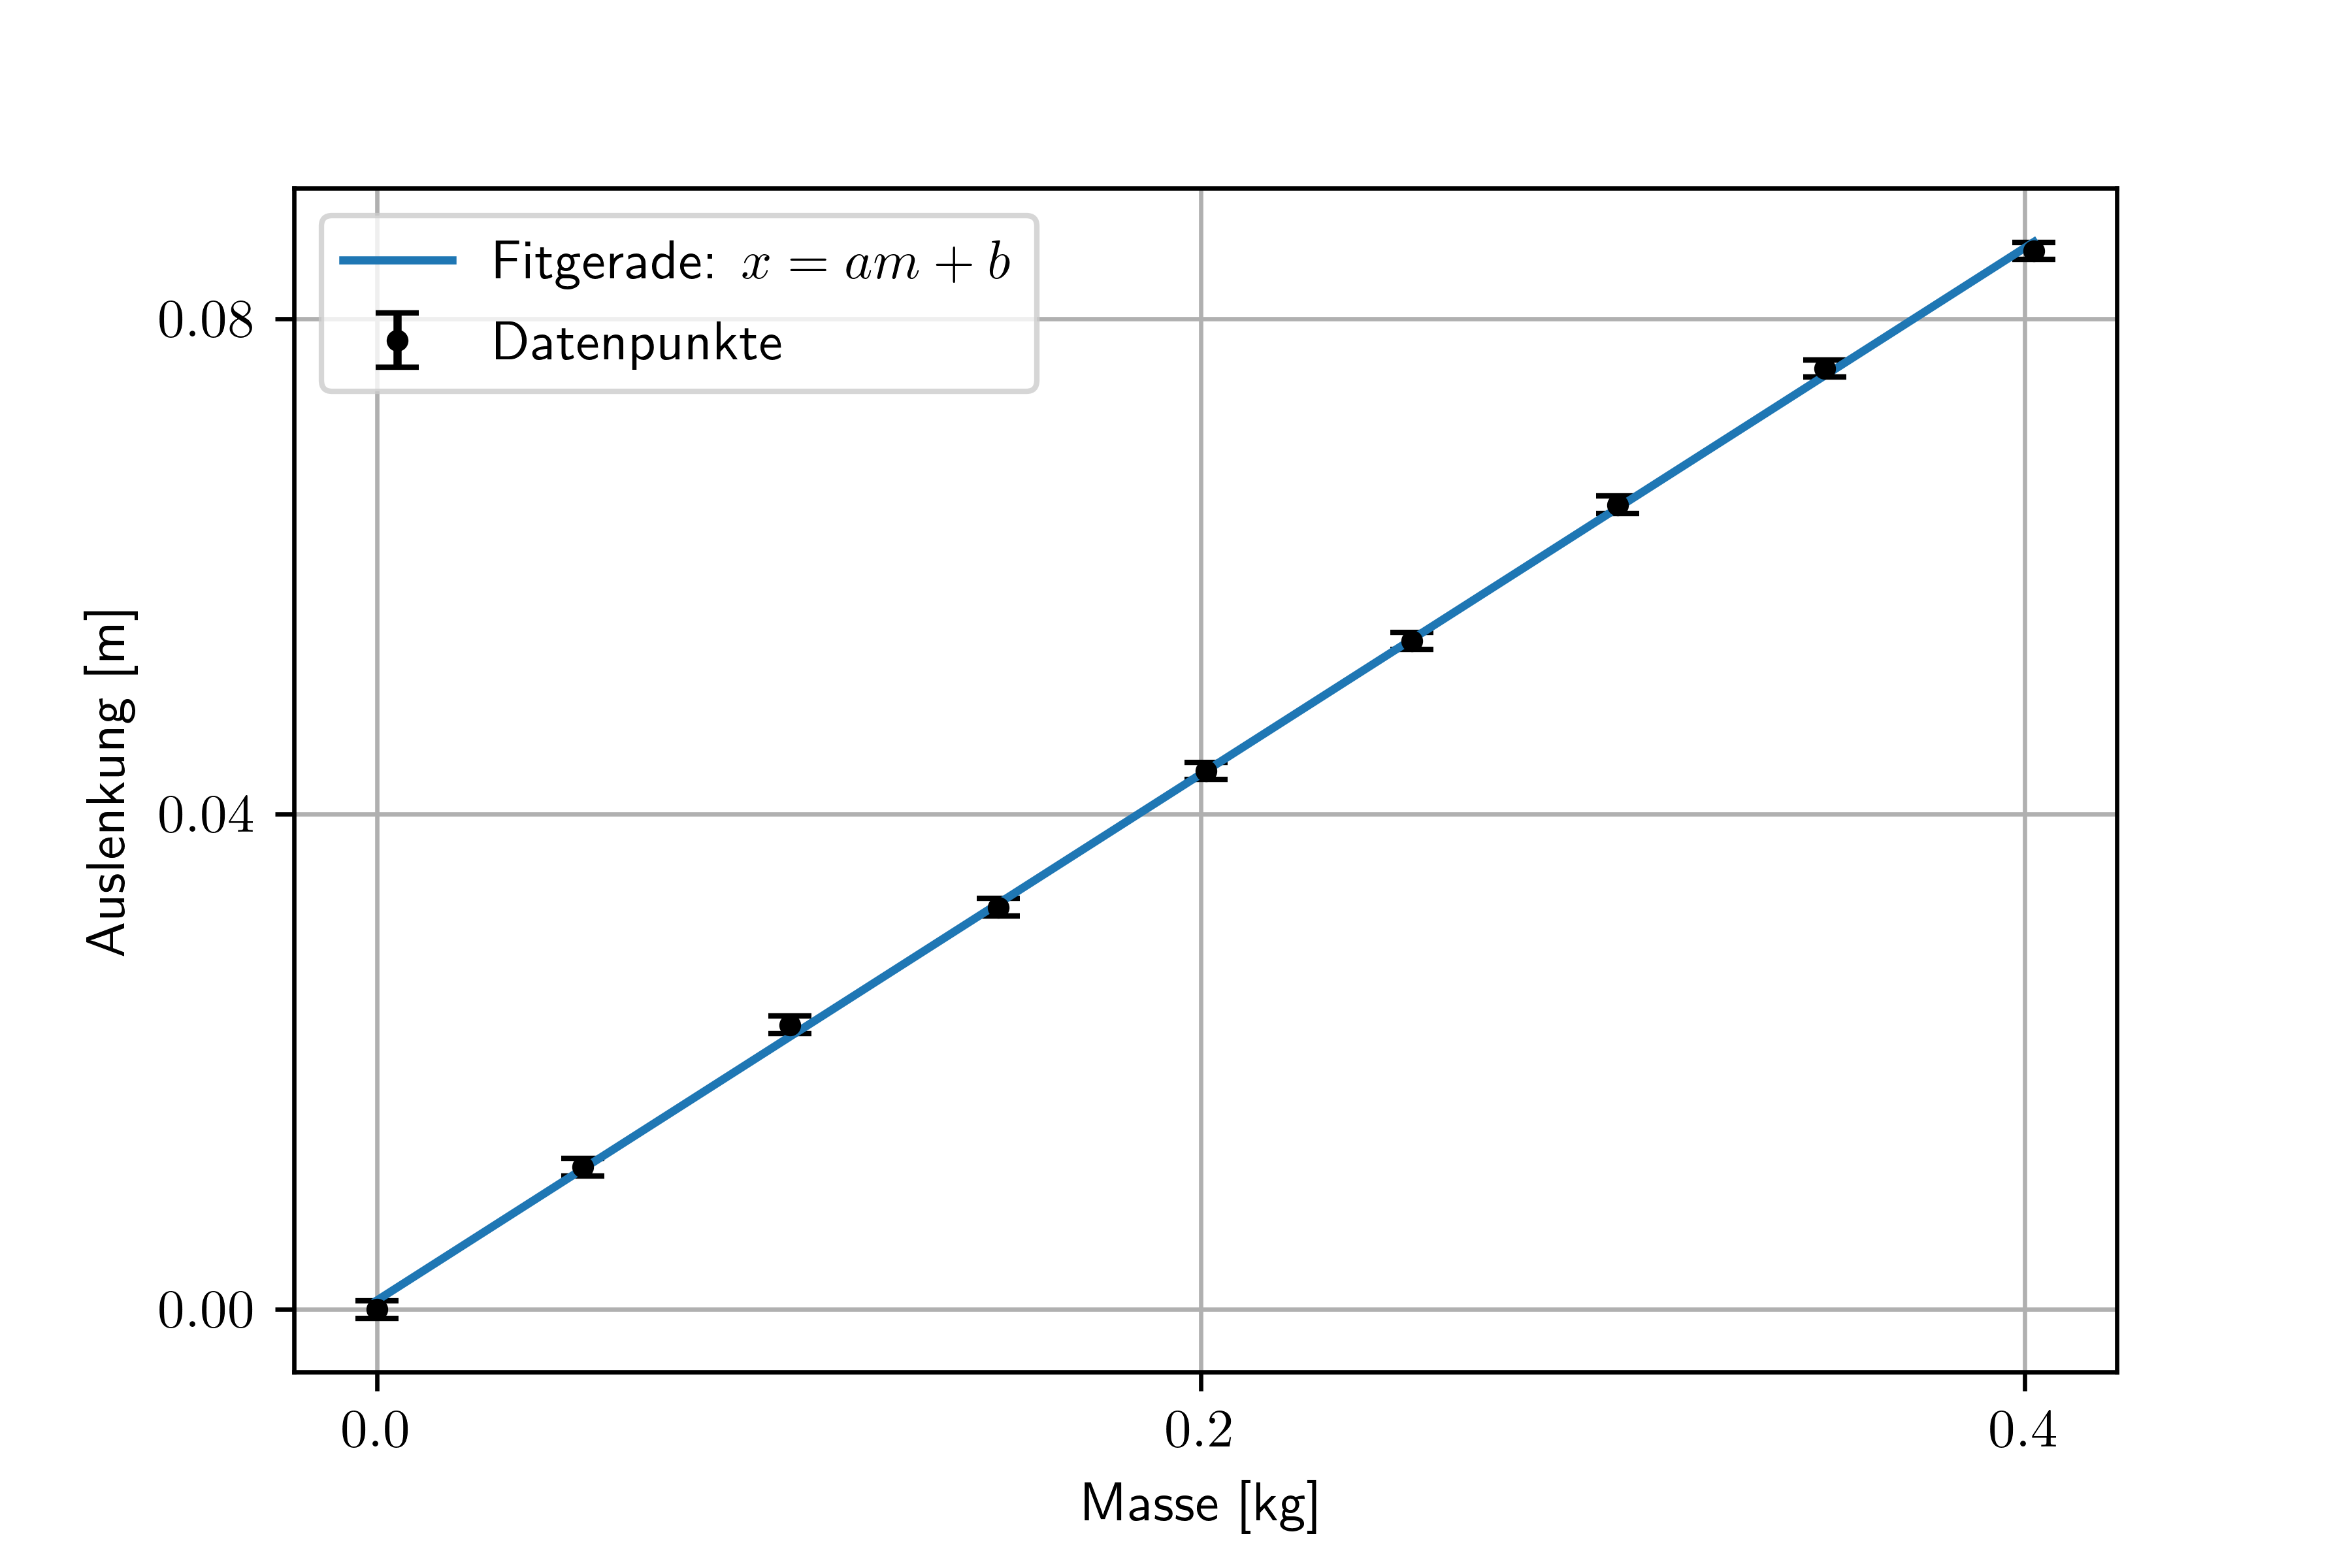
\includegraphics[width=350pt]{fotos/gpr1/B_Reg_A1_M1.png}			 
		\caption{Regeression, $ a=(0.2126\pm 0.0015) $, $ b=(7\pm 4)10^{-4} $}							 
		\label{Abb: Reg Ben A1 M1}							 
	\end{figure}
		\begin{figure}[!ht]
		\centering								 
		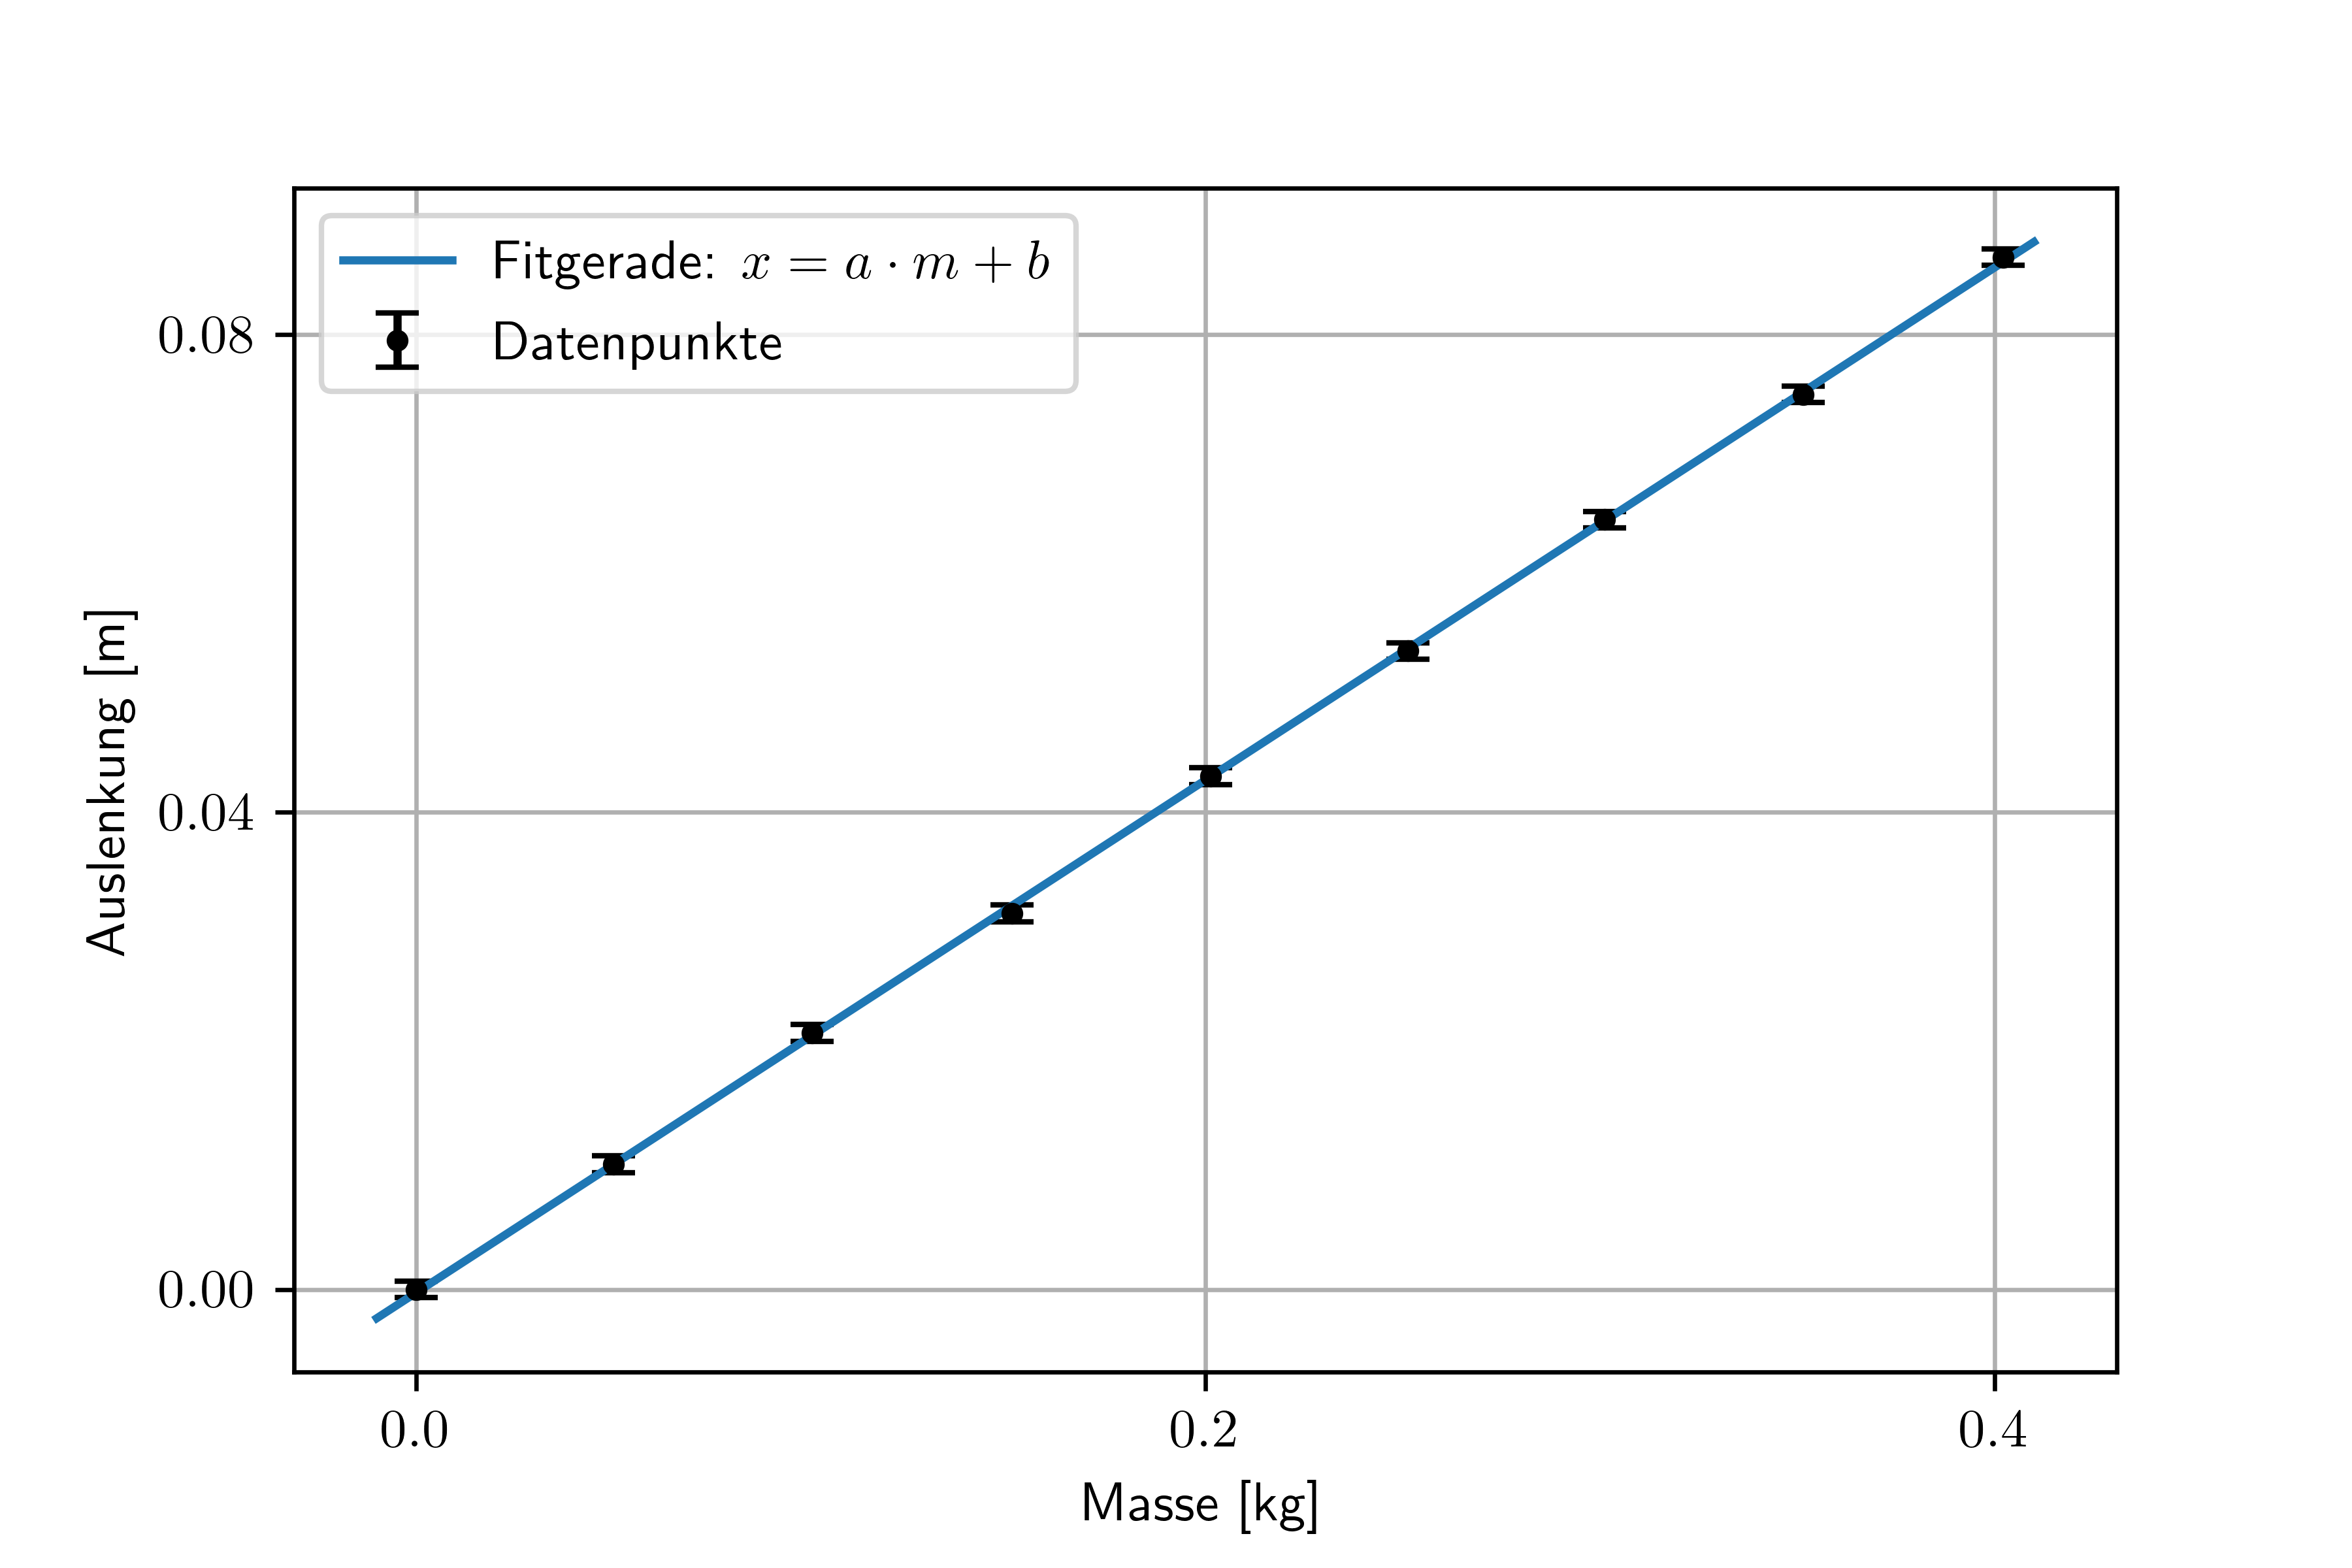
\includegraphics[width=350pt]{fotos/gpr1/B_Reg_A1_M2.png}			 
		\caption{Regeressionvon, $ a=(0.2147\pm 0.0009) $, $ b=(-2.6\pm 2.0)10^{-4} $}							 
		\label{Abb: Reg Ben A1 M2}							 
	\end{figure}
	\newpage
		\begin{figure}[!ht]
		\centering								 
		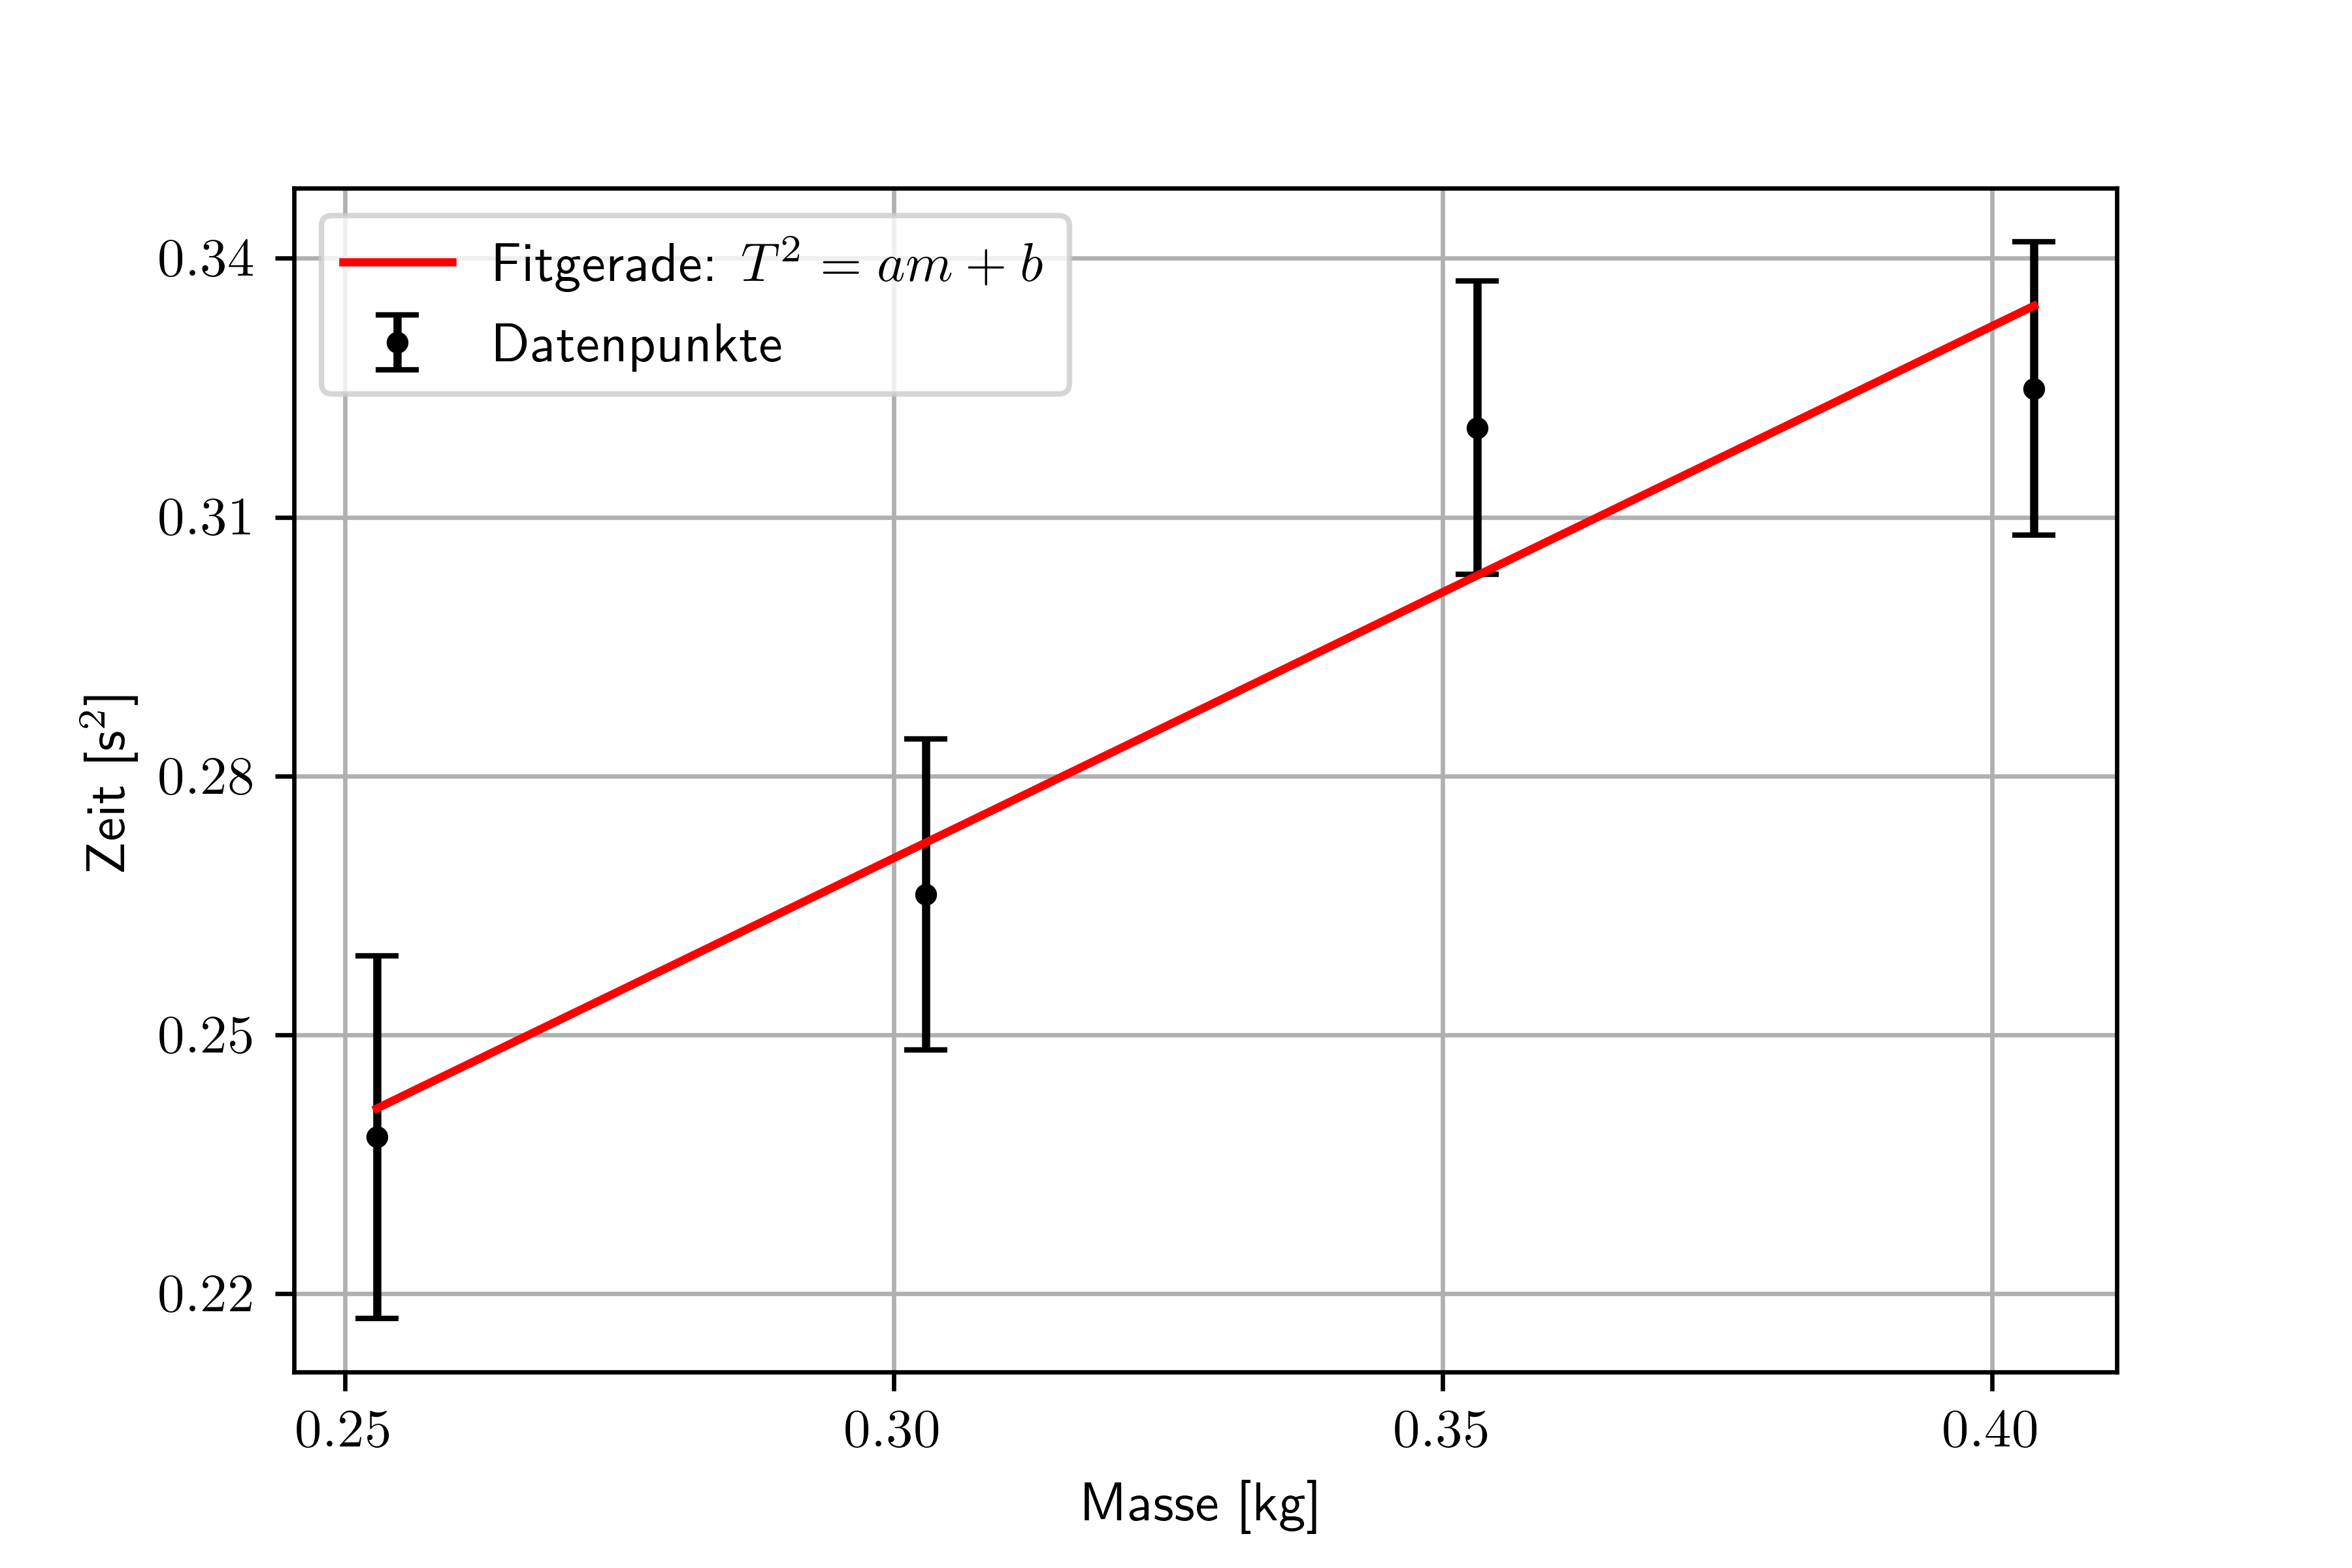
\includegraphics[width=350pt]{fotos/gpr1/B_Reg_A2.png}			 
		\caption{Regeressionvon, $ a=(0.00062\pm 0.00014) $, $ b=(9\pm 5)10^{-2} $ }							 
		\label{Abb: Reg Ben A2}							 
	\end{figure}
		\begin{figure}[!ht]
		\centering								 
		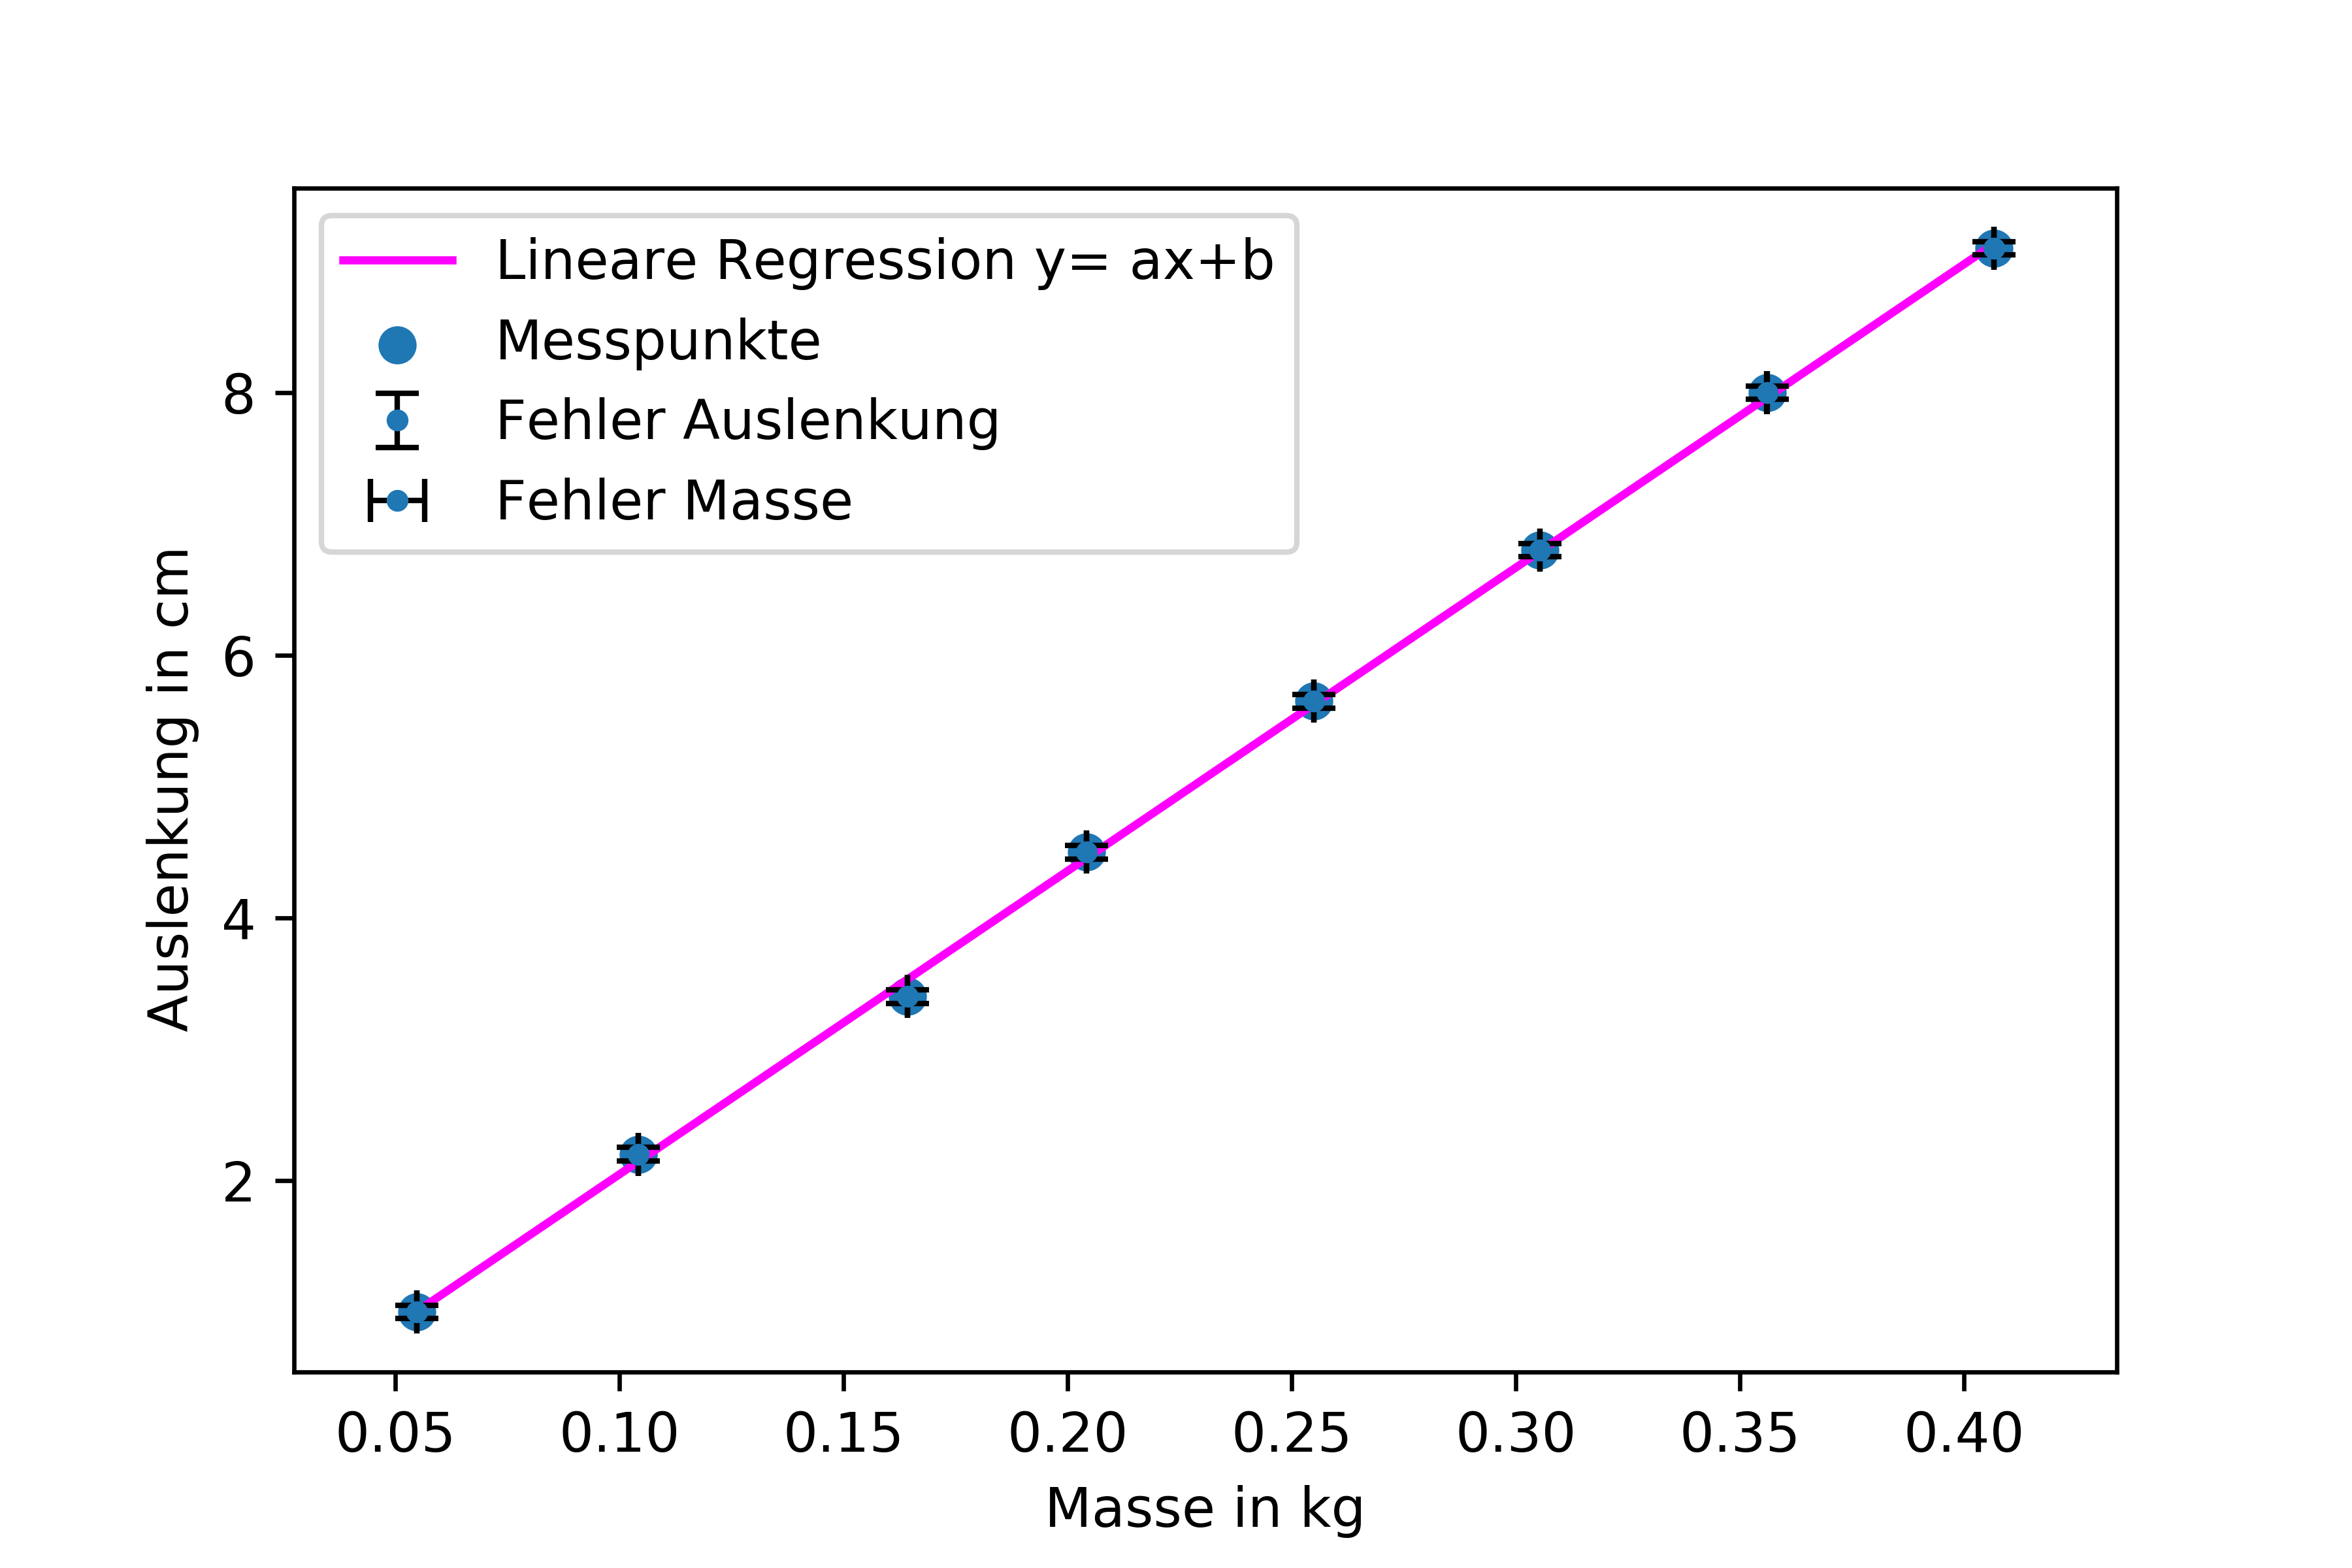
\includegraphics[width=350pt]{fotos/gpr1/S_Reg_A1.png}			 
		\caption{Regeressionvon, $ a=(23.11\pm 0.2)\text{ cm kg}^{-1} $, $ b= $}							 
		\label{Abb: Reg Sara A1}							 
	\end{figure}
	\newpage
		\begin{figure}[!ht]
		\centering								 
		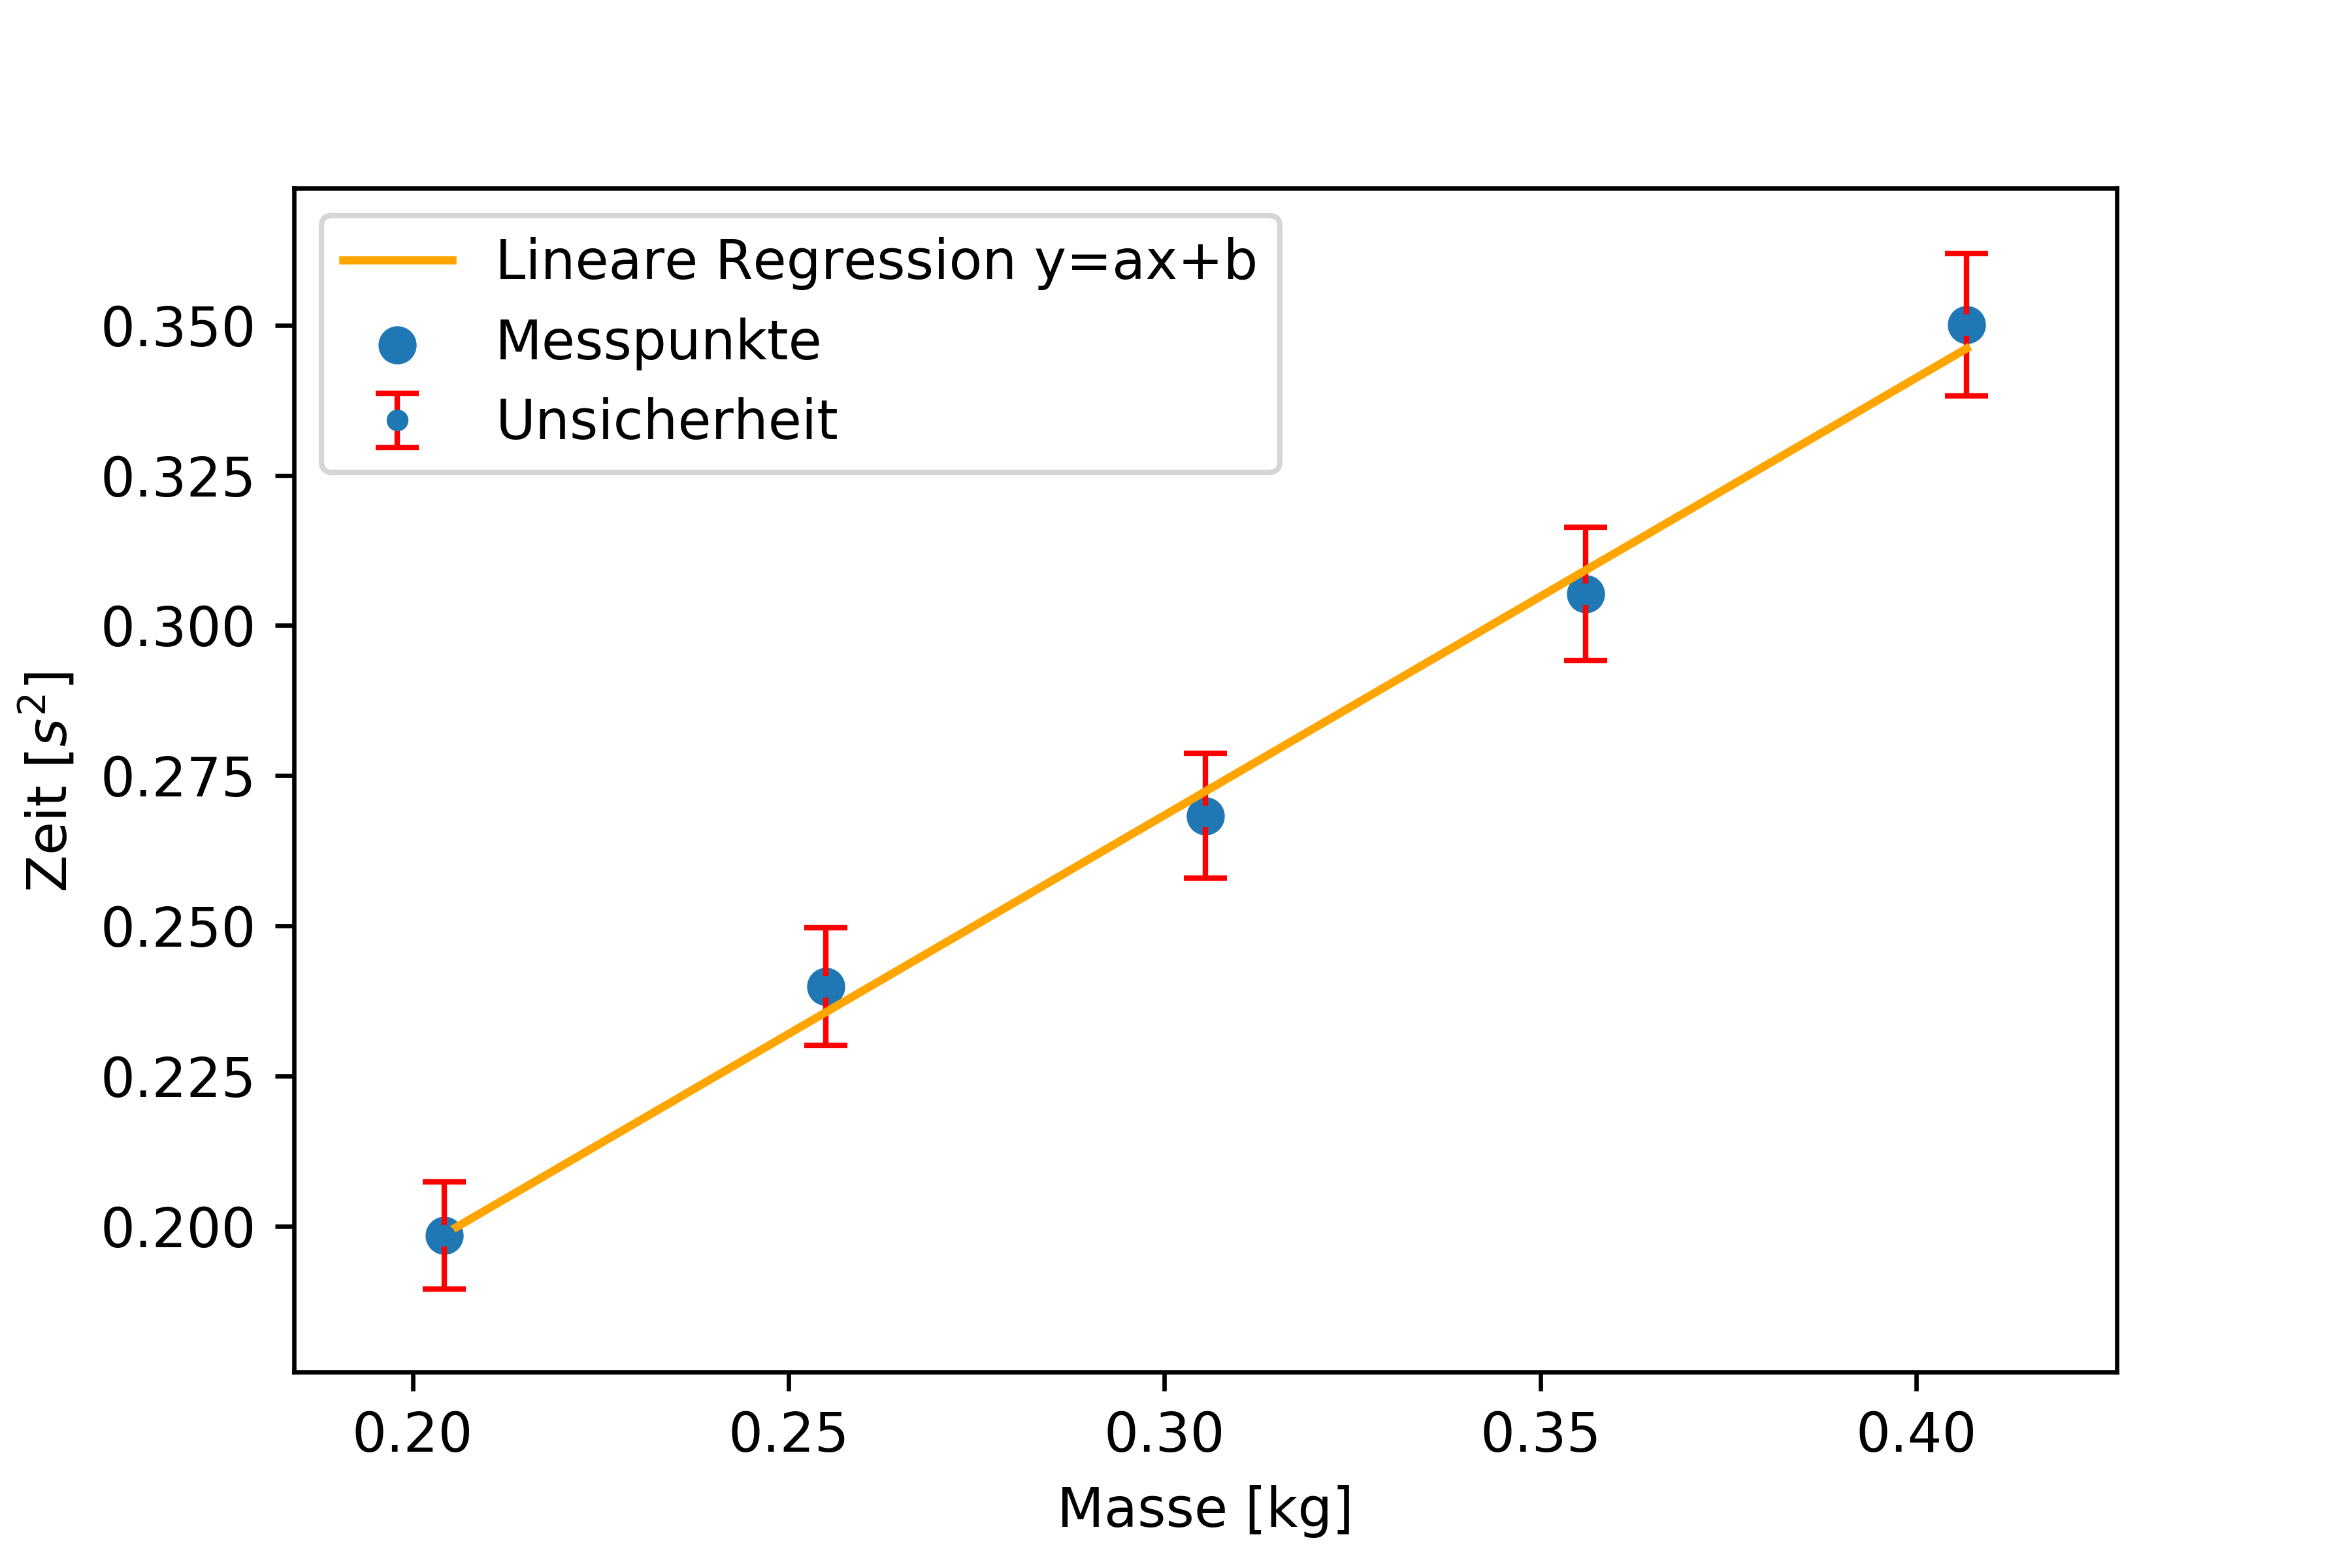
\includegraphics[width=350pt]{fotos/gpr1/S_Reg_A2.png}			 
		\caption{Regeression, S. }							 
		\label{Abb: Reg Sara A2}							 
	\end{figure}
\subsection{Chi-Quadrat Grafiken}
\begin{figure}[!ht]
	\centering								 
	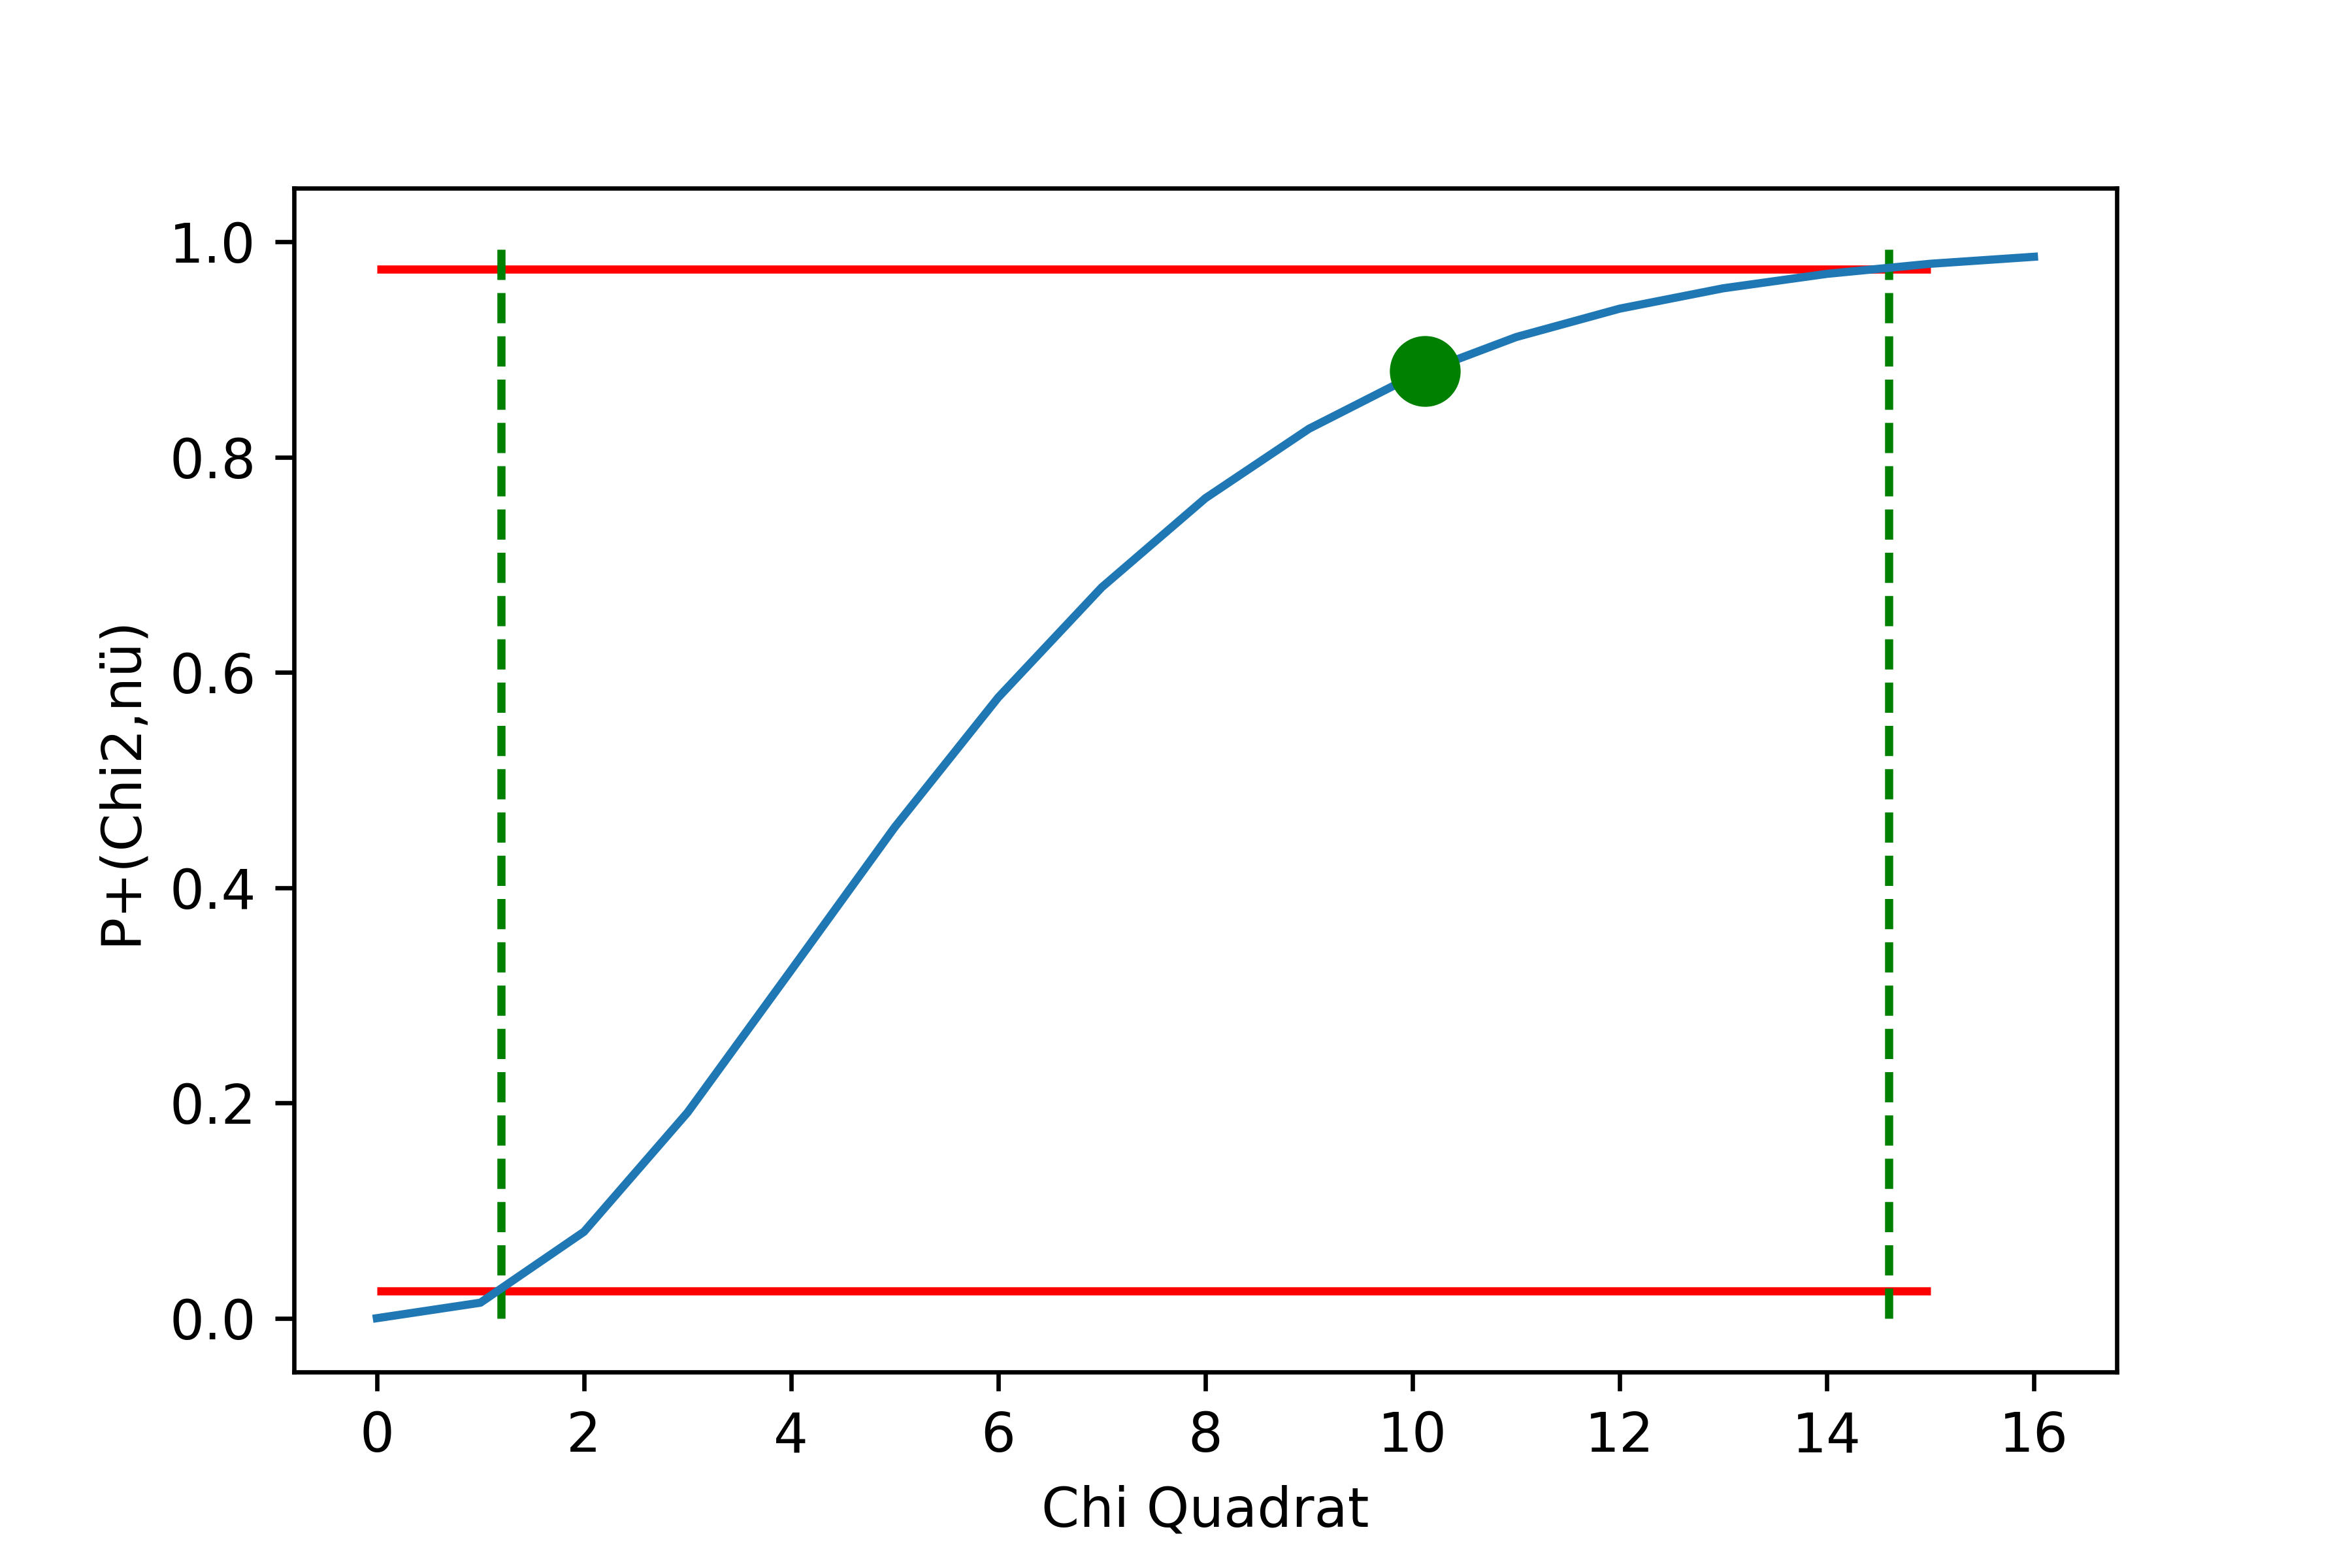
\includegraphics[width=350pt]{fotos/gpr1/kumulierte Chi Quadrat Verteilung V1.png}			 
	\caption{kumulierte Chi Quadrat Verteilung V1}							 
	\label{kumulierte Chi Quadrat Verteilung V1}							 
\end{figure}
\newpage
\begin{figure}[!ht]
	\centering								 
	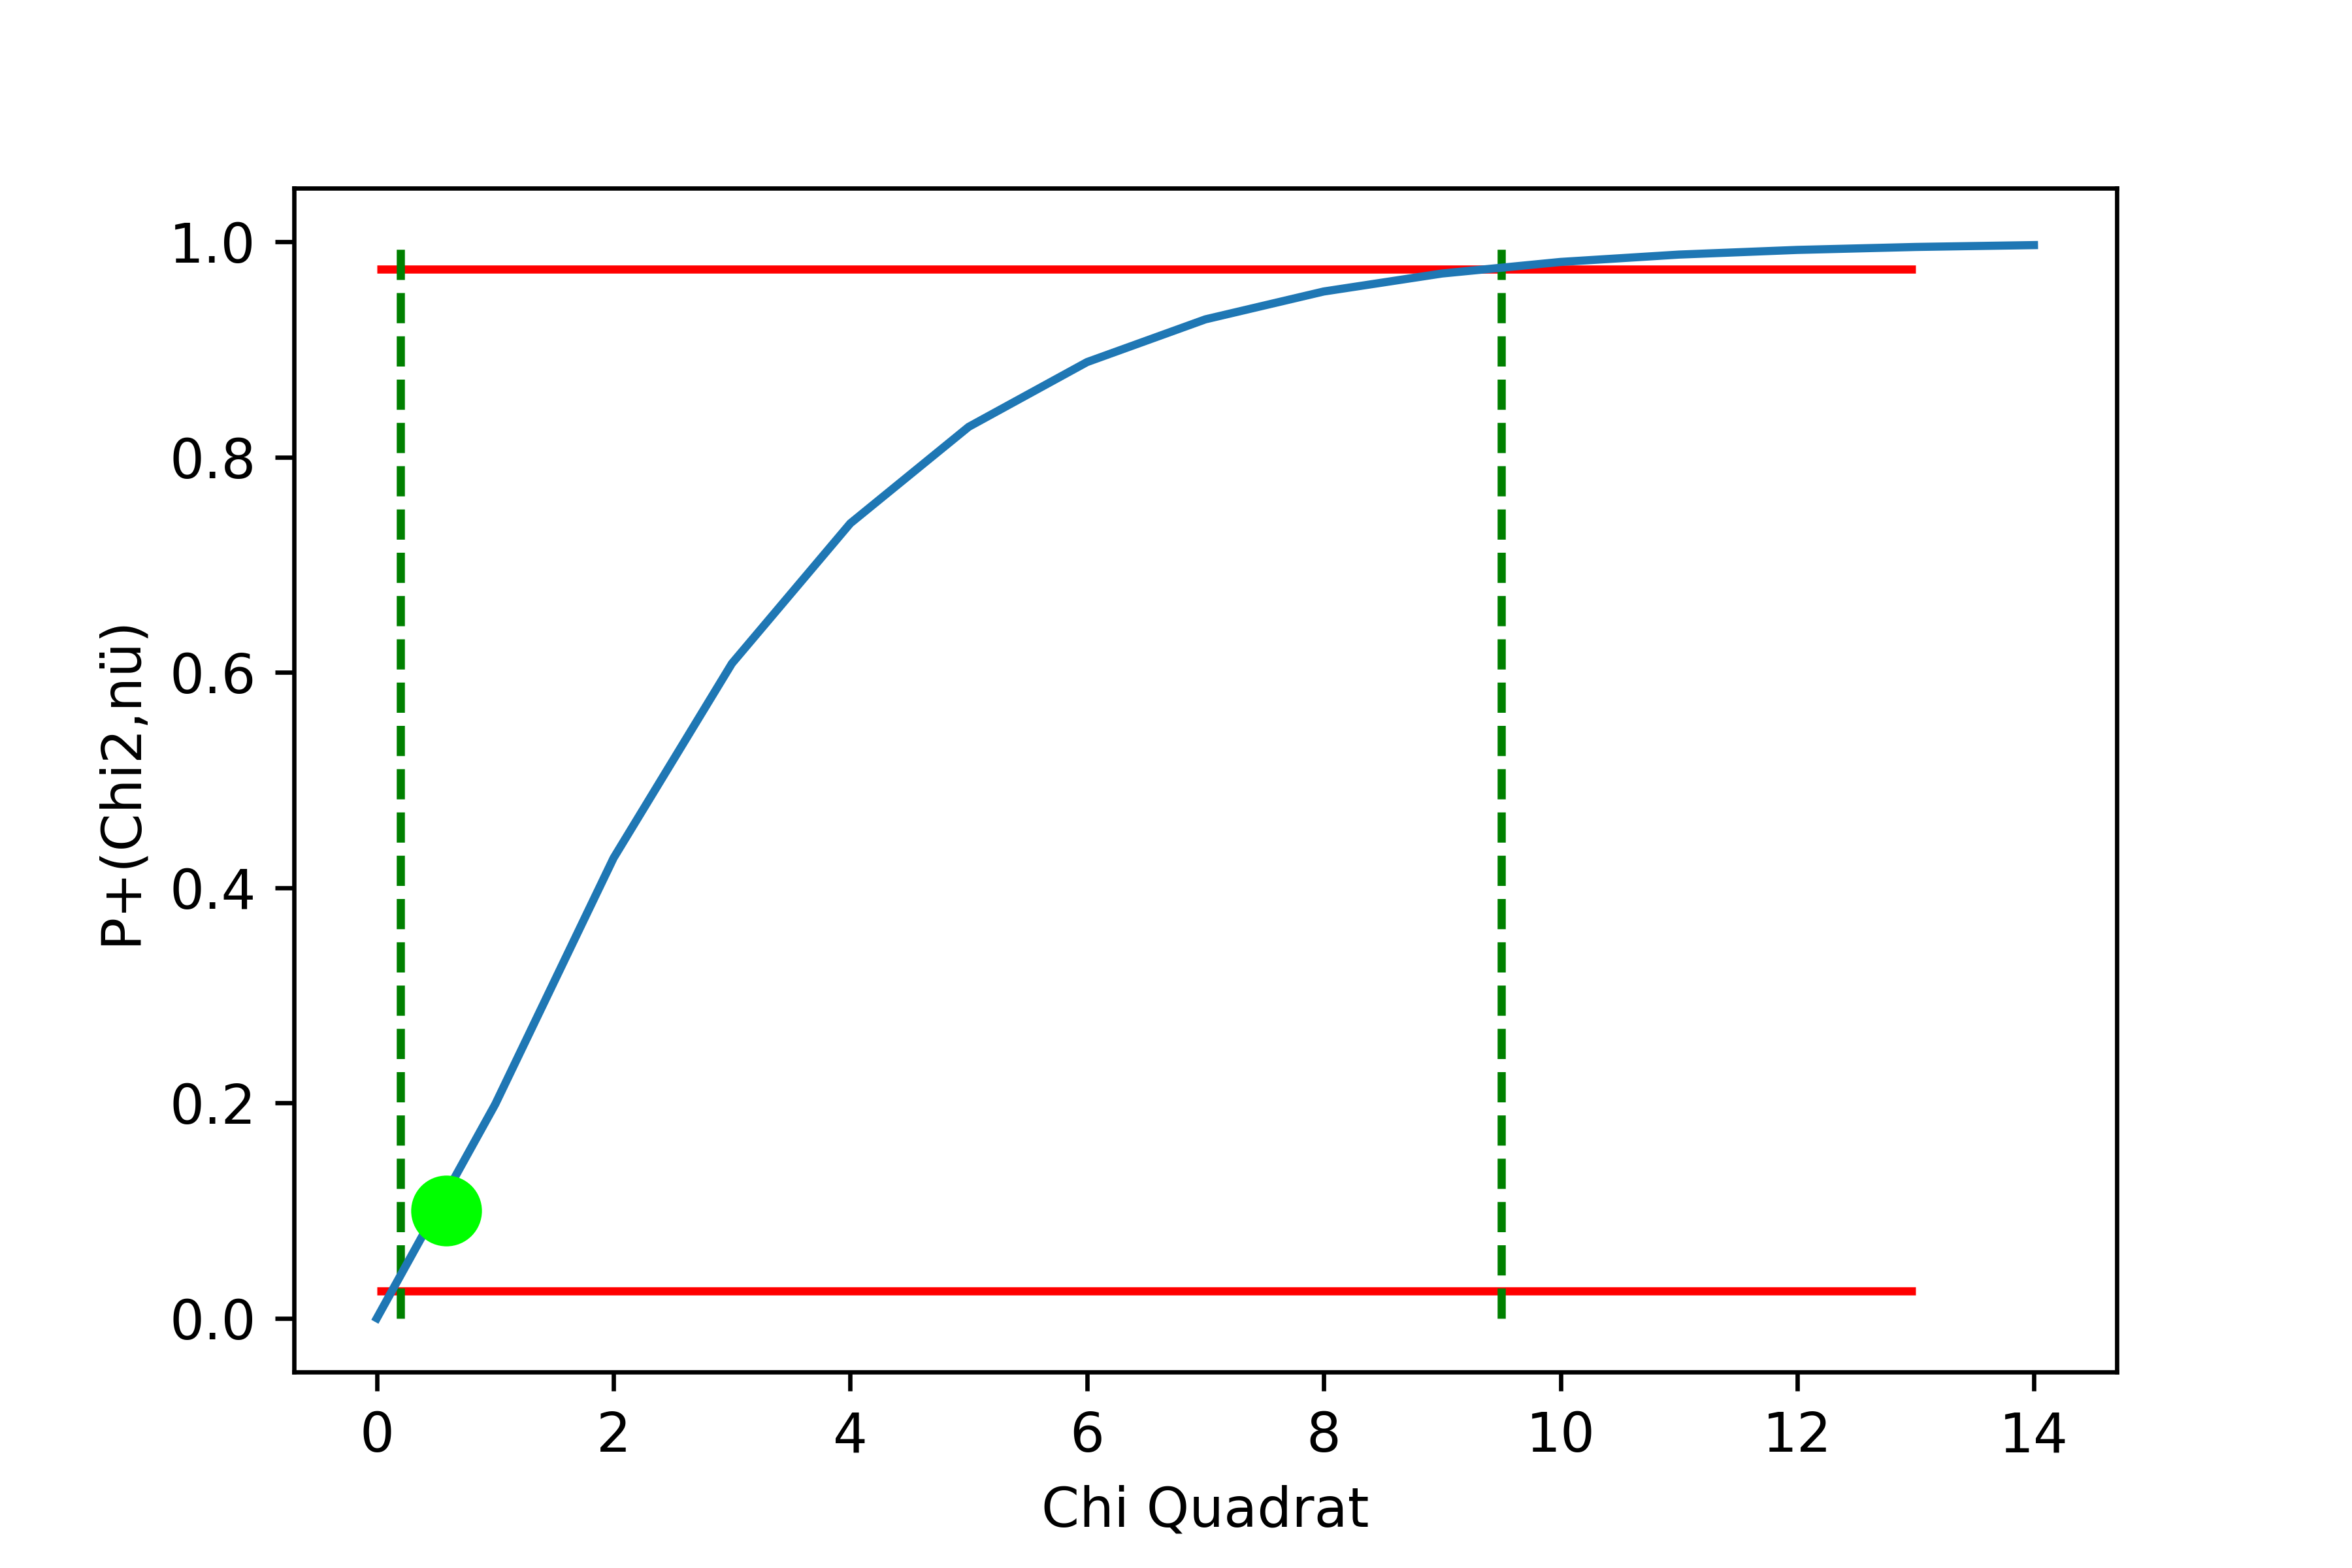
\includegraphics[width=350pt]{fotos/gpr1/kumulierte Chi Quadrat Verteilung V2.png}			 
	\caption{kumulierte Chi Quadrat Verteilung V2}							 
	\label{kumulierte Chi Quadrat Verteilung V2}							 
\end{figure}

\begin{figure}[!ht]
	\centering								 
	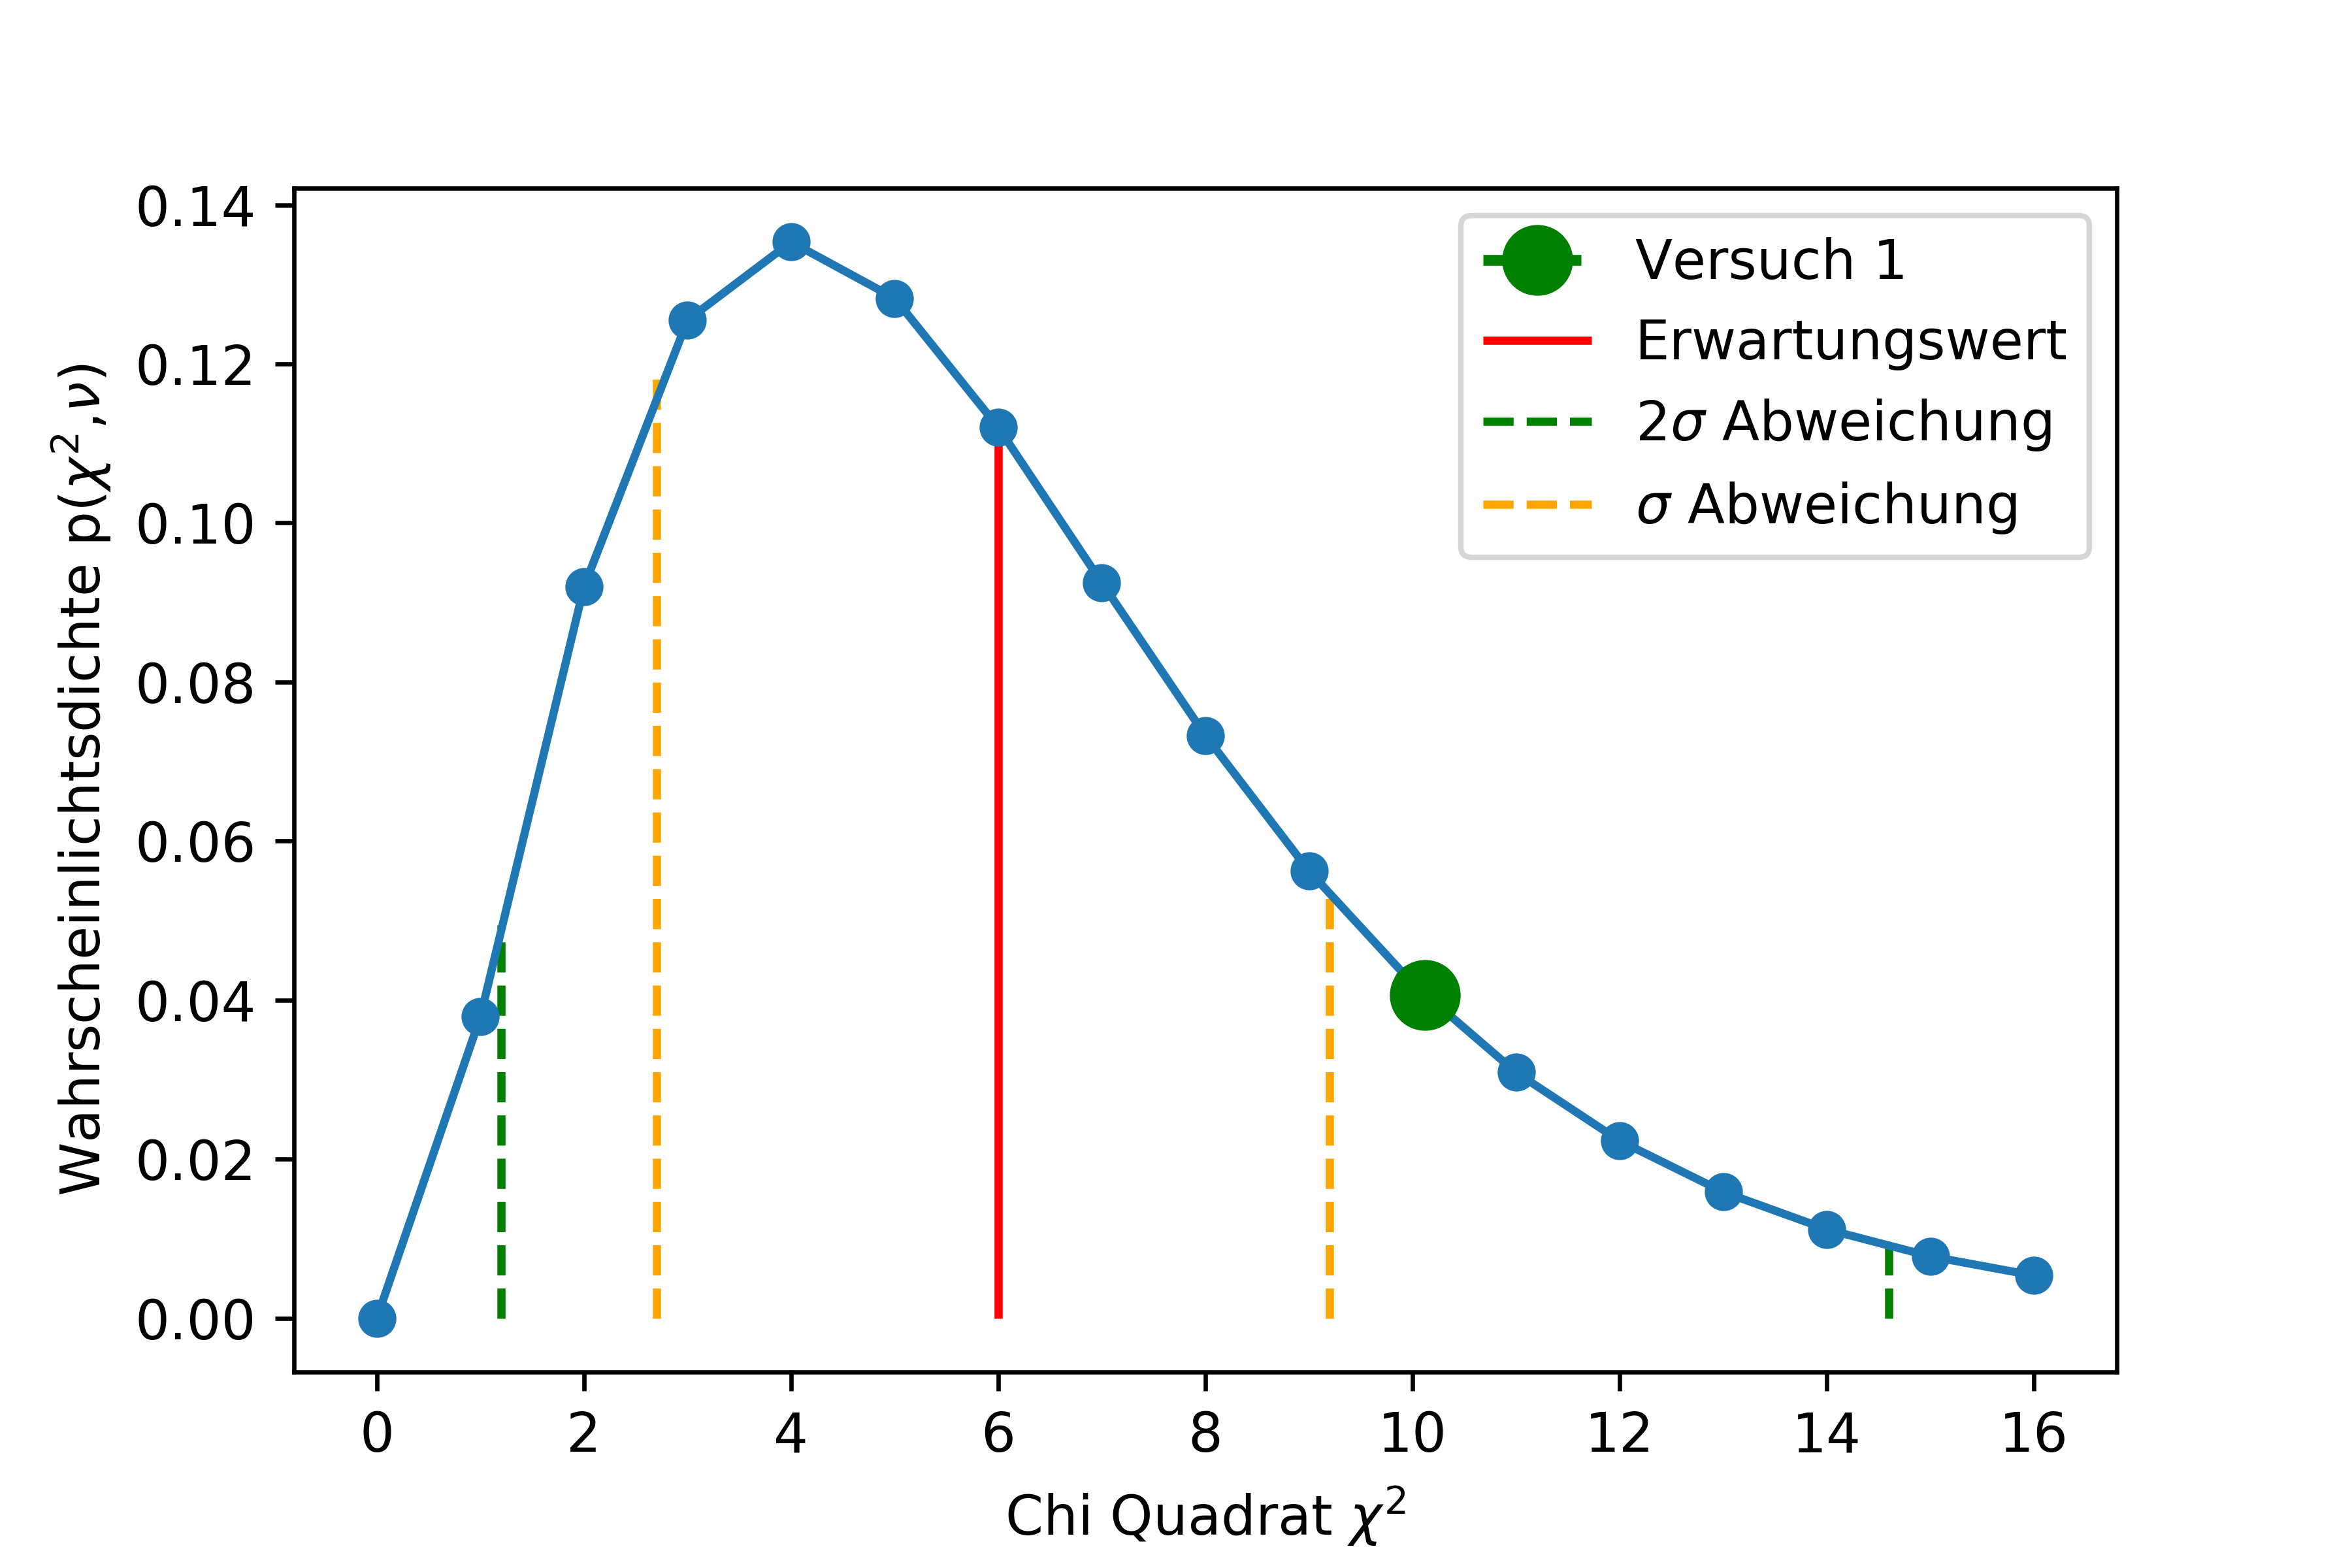
\includegraphics[width=350pt]{fotos/gpr1/Chi-Quadrat Wahrscheinlichkeitsdichte V1.png}			 
	\caption{Chi-Quadrat Wahrscheinlichkeitsdichte V1}							 
	\label{Chi-Quadrat Wahrscheinlichkeitsdichte V1}							 
\end{figure}
\newpage
\begin{figure}[!ht]
	\centering								 
	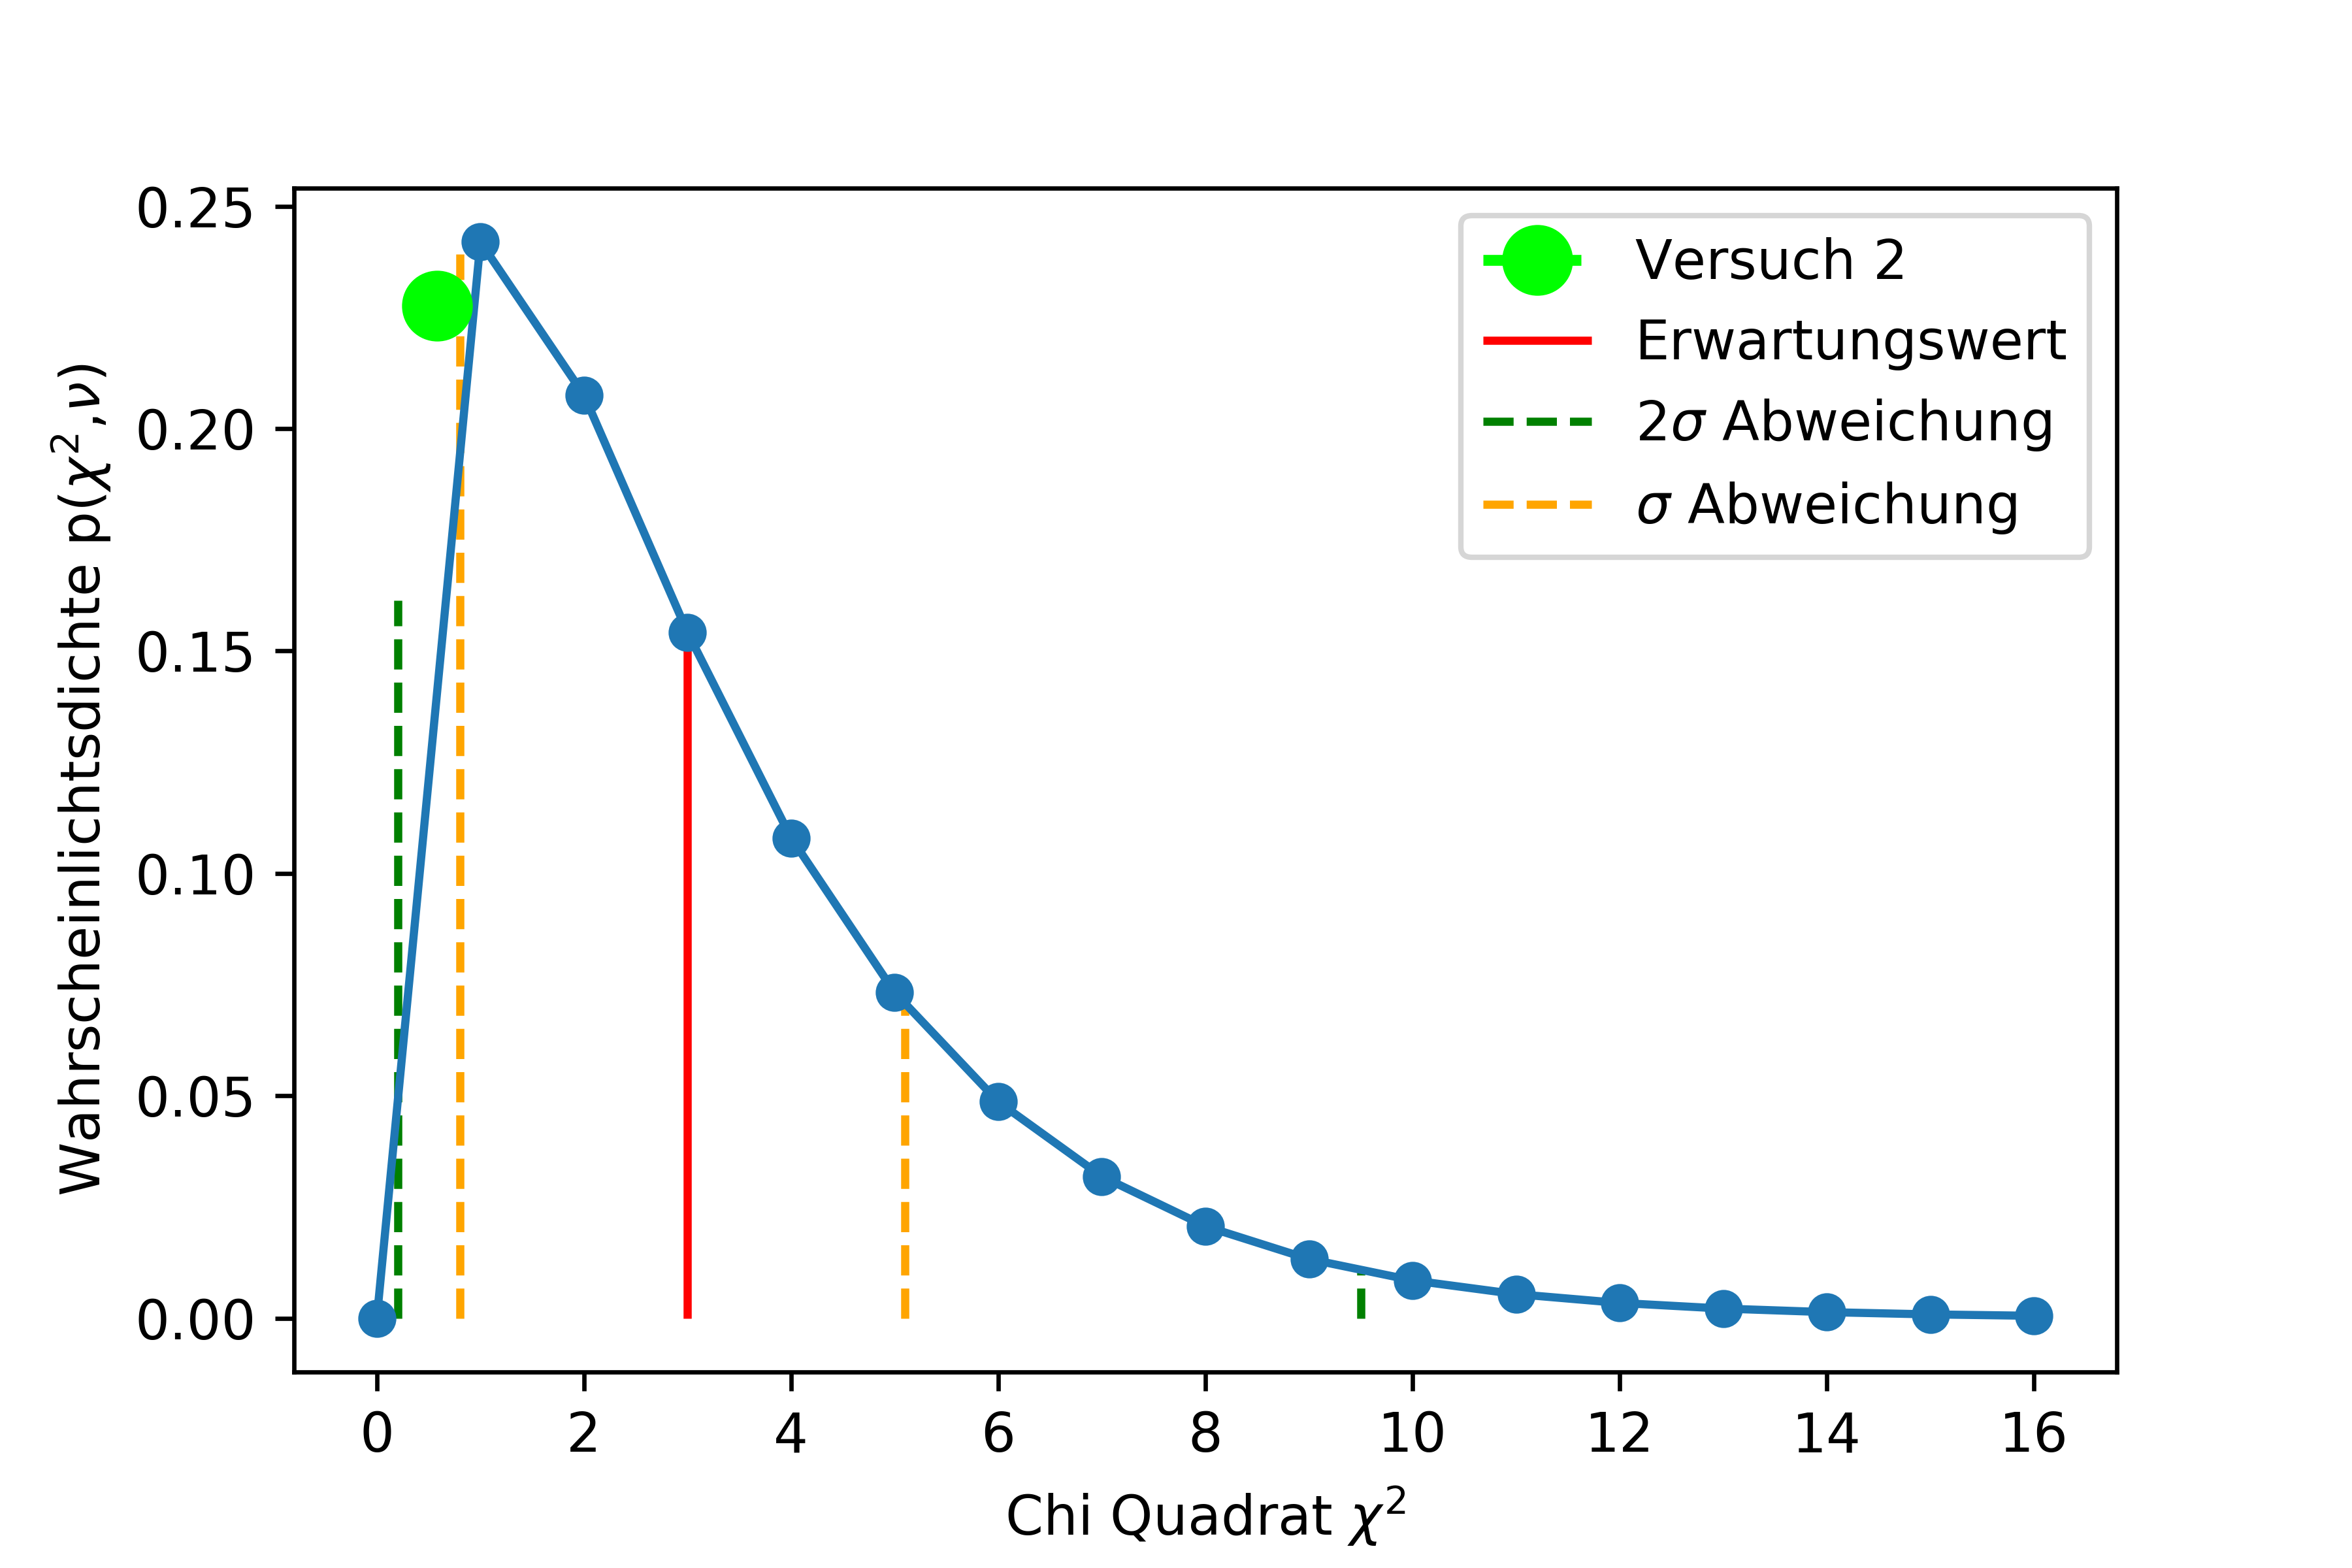
\includegraphics[width=350pt]{fotos/gpr1/Chi-Quadrat Wahrscheinlichkeitsdichte V2.png}			 
	\caption{Chi-Quadrat Wahrscheinlichkeitsdichte V2}							 
	\label{Chi-Quadrat Wahrscheinlichkeitsdichte V2}							 
\end{figure}
\begin{figure}[!ht]
	\centering								 
	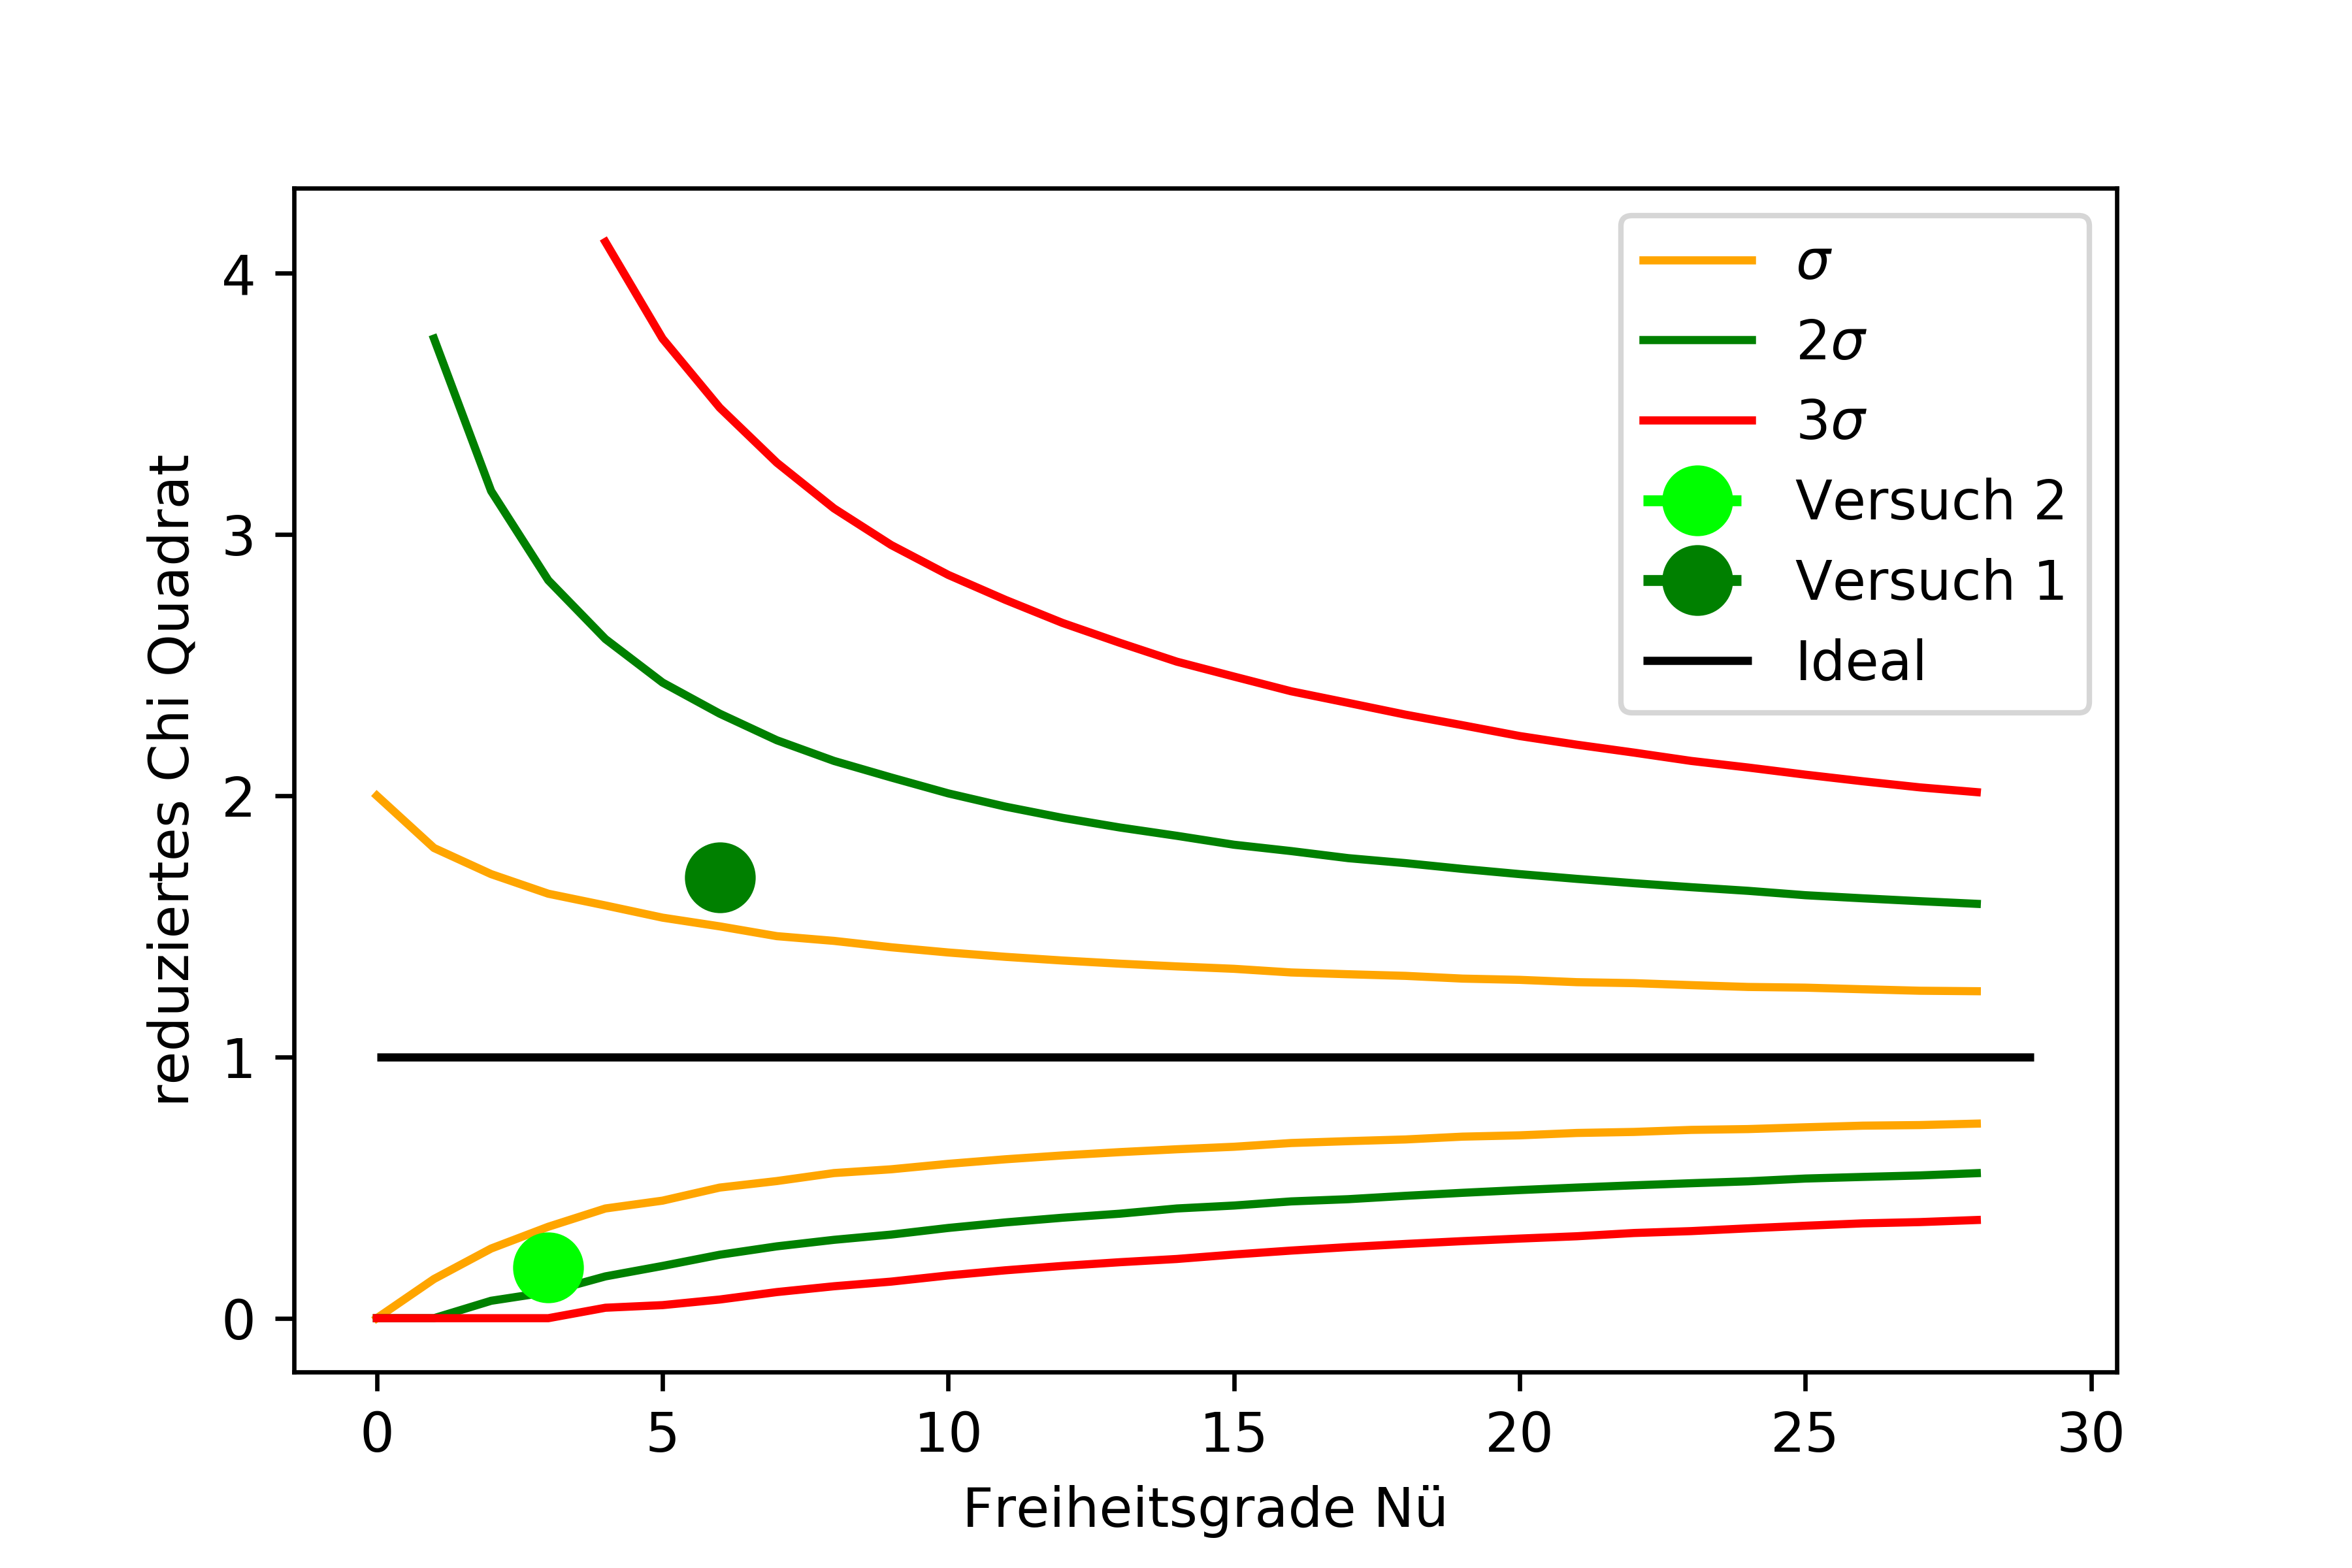
\includegraphics[width=350pt]{fotos/gpr1/Konfidenzintervall vs Freiheitsgrade im reduzierten Chi Quadrat.png}			 
	\caption{Konfidenzintervall vs Freiheitsgrade im reduzierten Chi Quadrat}							 
	\label{Konfidenzintervall vs Freiheitsgrade im reduzierten Chi Quadrat}							 
\end{figure}

